\documentclass[11pt]{article}

\usepackage[margin=0.88in]{geometry}
\usepackage[T1]{fontenc}
\usepackage[utf8]{inputenc}
\usepackage{lmodern}
\usepackage{microtype}
\usepackage{amsmath,amssymb,amsthm,mathtools,bm}
\usepackage{booktabs,array,tabularx,longtable,multirow}
\usepackage{graphicx}
\usepackage{enumitem}
\usepackage{xcolor}
\usepackage{caption}
\usepackage{subcaption}
\usepackage{float}
\usepackage{setspace}
\usepackage{tikz}
\usetikzlibrary{arrows.meta,positioning,fit,calc,shapes.geometric,backgrounds}
\usepackage[most]{tcolorbox}
\usepackage{listings}
\usepackage{siunitx}
\usepackage[backend=biber,style=numeric-comp,sorting=none,maxbibnames=99]{biblatex}
\addbibresource{references.bib}
\graphicspath{{figures/}}
\usepackage[colorlinks=true,allcolors=blue!50!black]{hyperref}
\usepackage{aliascnt}
\usepackage[nameinlink,capitalise]{cleveref}

\hypersetup{
  pdftitle={CovQ: Certified Fisher-Information Contract Compilation for Commuting Pauli Programs},
  pdfauthor={Hina Chauhan Dixit},
  pdfsubject={Minimum-cost bounded-entanglement quantum programs from downstream Fisher-information floors},
  pdfkeywords={quantum compiler, Fisher-information contract, quantum Fisher information, commuting Pauli, matching polytope, Bell schedule, semidefinite optimization}
}

\setstretch{1.035}
\setlist{nosep,leftmargin=*}
\captionsetup{font=small,labelfont=bf}
\renewcommand{\arraystretch}{1.12}

\definecolor{covqteal}{HTML}{0C7489}
\definecolor{covqorange}{HTML}{C86A24}
\definecolor{covqgreen}{HTML}{2F7D32}
\definecolor{covqred}{HTML}{A33A3A}
\definecolor{covqgray}{HTML}{F2F3F4}
\definecolor{covqblue}{HTML}{365F91}

\newtheorem{theorem}{Theorem}[section]
\newaliascnt{proposition}{theorem}
\newtheorem{proposition}[proposition]{Proposition}
\aliascntresetthe{proposition}
\newaliascnt{lemma}{theorem}
\newtheorem{lemma}[lemma]{Lemma}
\aliascntresetthe{lemma}
\newaliascnt{corollary}{theorem}
\newtheorem{corollary}[corollary]{Corollary}
\aliascntresetthe{corollary}
\theoremstyle{definition}
\newaliascnt{definition}{theorem}
\newtheorem{definition}[definition]{Definition}
\aliascntresetthe{definition}
\newaliascnt{assumption}{theorem}
\newtheorem{assumption}[assumption]{Assumption}
\aliascntresetthe{assumption}
\newaliascnt{problem}{theorem}
\newtheorem{problem}[problem]{Problem}
\aliascntresetthe{problem}
\theoremstyle{remark}
\newaliascnt{remark}{theorem}
\newtheorem{remark}[remark]{Remark}
\aliascntresetthe{remark}
\newaliascnt{example}{theorem}
\newtheorem{example}[example]{Example}
\aliascntresetthe{example}

\crefname{theorem}{theorem}{theorems}
\crefname{proposition}{proposition}{propositions}
\crefname{lemma}{lemma}{lemmas}
\crefname{corollary}{corollary}{corollaries}
\crefname{definition}{definition}{definitions}
\crefname{assumption}{assumption}{assumptions}
\crefname{problem}{problem}{problems}
\crefname{remark}{remark}{remarks}
\crefname{example}{example}{examples}

\newcommand{\R}{\mathbb{R}}
\newcommand{\C}{\mathbb{C}}
\newcommand{\F}{\mathsf{F}}
\newcommand{\Q}{\mathcal{Q}}
\newcommand{\G}{\mathcal{G}}
\newcommand{\Hh}{\mathcal{H}}
\newcommand{\PiProg}{\mathsf{\Pi}}
\newcommand{\MATCH}{\operatorname{MATCH}}
\newcommand{\CUT}{\operatorname{CUT}}
\newcommand{\Cov}{\operatorname{Cov}}
\newcommand{\Var}{\operatorname{Var}}
\newcommand{\diag}{\operatorname{diag}}
\newcommand{\rank}{\operatorname{rank}}
\newcommand{\tr}{\operatorname{tr}}
\newcommand{\supp}{\operatorname{supp}}
\newcommand{\conv}{\operatorname{conv}}
\newcommand{\dist}{\operatorname{dist}}
\newcommand{\cone}{\operatorname{cone}}
\newcommand{\sgn}{\operatorname{sgn}}
\newcommand{\poly}{\operatorname{poly}}
\newcommand{\kernel}{\operatorname{ker}}
\newcommand{\im}{\operatorname{Im}}
\newcommand{\off}{\operatorname{off}}
\newcommand{\op}{\mathrm{op}}
\newcommand{\cq}{\mathrm{CQ}}
\newcommand{\coh}{\mathrm{coh}}
\newcommand{\deph}{\mathrm{deph}}
\newcommand{\lab}{\mathrm{lab}}
\newcommand{\phys}{\mathrm{phys}}
\newcommand{\logical}{\mathrm{log}}
\newcommand{\dd}{\,\mathrm{d}}
\newcommand{\ket}[1]{\lvert #1\rangle}
\newcommand{\bra}[1]{\langle #1\rvert}
\newcommand{\braket}[2]{\langle #1\mid #2\rangle}
\newcommand{\proj}[1]{\lvert #1\rangle\!\langle #1\rvert}
\newcommand{\inner}[2]{\left\langle #1,#2\right\rangle}
\newcommand{\ones}{\mathbf{1}}
\newcommand{\eps}{\varepsilon}
\newcommand{\Cost}{\operatorname{Cost}}
\newcommand{\OPT}{\operatorname{OPT}}
\newcommand{\suppfun}{\operatorname{h}}
\newcommand{\placeholder}[1]{\begin{tcolorbox}[colback=covqgray,colframe=covqorange,title={Repository result pending}]#1\end{tcolorbox}}

\newtcolorbox{claimbox}[1][]{
  colback=covqgray,
  colframe=covqteal,
  boxrule=0.8pt,
  arc=1.5mm,
  left=2mm,right=2mm,top=1.5mm,bottom=1.5mm,
  #1
}
\newtcolorbox{warningbox}[1][]{
  colback=red!3,
  colframe=covqred,
  boxrule=0.8pt,
  arc=1.5mm,
  left=2mm,right=2mm,top=1.5mm,bottom=1.5mm,
  #1
}
\newtcolorbox{methodbox}[1][]{
  colback=blue!2,
  colframe=covqblue,
  boxrule=0.8pt,
  arc=1.5mm,
  left=2mm,right=2mm,top=1.5mm,bottom=1.5mm,
  #1
}

\lstdefinestyle{covqcode}{
  basicstyle=\ttfamily\footnotesize,
  backgroundcolor=\color{covqgray},
  frame=single,
  rulecolor=\color{black!20},
  breaklines=true,
  columns=fullflexible,
  showstringspaces=false
}

\title{\textbf{CovQ: Certified Fisher-Information Contract Compilation\\for Commuting Pauli Programs}\\[0.35em]
\large Exact Pair-Width Geometry, Operational Readout,\\and Noise-Aware Hardware-Native Bell Schedules}
\author{Hina Chauhan Dixit\\Decompute Inc.}
\date{Journal-preparation manuscript v0.4 --- August 2026}

\begin{document}
\maketitle

\begin{abstract}
A downstream quantum-estimation task rarely requires one prescribed state or one prescribed quantum Fisher information matrix (QFIM). It requires enough information about specified parameter combinations at acceptable experimental cost. We introduce \emph{CovQ}, a compiler for that contract. Given commuting Pauli generators $\G$, a hardware graph $H$, a downstream map $A$, a required Fisher-information floor $G_{\rm req}\succeq0$, and a declared cost model, CovQ emits an exposure-weighted retained-label program, hardware-native preparation circuits, an ancilla-free local readout, an estimator, and primal--dual certificates satisfying
\[
  \sum_b n_b A^{\mathsf T}F_{C,b}A\succeq G_{\rm req}.
\]
Exact QFIM matching remains a verification and interoperability mode rather than the sole compiler purpose.

The mathematical engine is an exact reachable-body theorem for labeled pair-entangled programs. For physical $Z_i/2$ generators on a native graph $H=(V,E)$, a unit-diagonal matrix $F$ is achievable with width-two branches if and only if its nonedge entries vanish and $(|F_{ij}|)_{ij\in E}$ lies in Edmonds' matching polytope. This identification is quantum rather than merely combinatorial: every width-two branch induces a signed matching; edge signs are independently realizable; every matching-polytope point becomes a retained-label schedule of parallel signed Bell pairs; and the emitted schedule attains the complete matrix. It yields a convex fixed-exposure compiler and a homogenized shot-scaled compiler. Their dual circuit constraints are separated exactly by maximum-weight matching, while numerical conic optimization is certified to prescribed accuracy.

For every emitted signed-cat block, a product of single-qubit equatorial measurements attains the ideal QFIM; no ancilla or joint Bell measurement is required. The block parity is sufficient, a branch-conditioned maximum-likelihood estimator is consistent and empirically efficient, and a two-quadrature pilot identifies the correct periodic likelihood chart. Under phase-covariant dephasing, matched quadrature attains the mixed-state QFIM $v^2ss^{\mathsf T}$. In contrast, pinching in the joint generator eigenbasis preserves every generator covariance while driving both QFI and operational information to zero.

Block-local noise preserves the compiler's combinatorics. Every nonempty branch becomes a shared depth-one idling template plus independent signed edge increments, so noisy reduced-cost pricing remains maximum-weight matching, supplemented by a separately priced zero-depth product column. The pricing oracle agreed with exhaustive signed-matching enumeration in all 12 registered cases to $4.4\times10^{-16}$, and primal--dual gaps were below $10^{-15}$. The compiler changed its program under noise, abandoning all entangled branches between the registered edge-depolarization levels $0.15$ and $0.20$.

Against a faithful QUEST reimplementation on exact targets, CovQ retained two-qubit preparation depth one, while QUEST required factors of $2.5$--$135.6$ more CX gates than CovQ's expected count on the ten converged instances, while paying additional settings; one harder path instance reached the QUEST depth cap. In an equal-accounting noisy contract case, QUEST's optimistic QFI bound required less exposure at zero two-qubit noise (1.626 versus 1.766), but CovQ's emitted-readout classical Fisher information required less exposure at every tested point from $1\%$ edge depolarization onward; at $20\%$, the values were 2.759 versus $3.51\times10^5$. A fixed-setting greedy extension failed by $7.24\%$ in the multi-setting regime and is retained as a negative result. These measurements support a regime statement, not universal superiority: one-state preparation wins when coherence is cheap, whereas certified depth-one schedules become preferable when deep preparation is sufficiently noisy and repeated execution amortizes reconfiguration.
\end{abstract}

\noindent\textbf{Keywords:} quantum compilation; Fisher-information contracts; quantum Fisher information; commuting Pauli programs; matching polytope; Bell-state schedules; semidefinite optimization; hardware-aware synthesis.

\begin{claimbox}[title={Evidentiary status and release boundary}]
The theorem, proposition, lemma, and corollary statements are proved in this manuscript; classical correlation and matching results are attributed. The implementation results reported below are drawn from repository commit \texttt{6a5b526} and its committed canonical records, with 156 tests passing. Those records still carry pre-commit \texttt{source\_commit} fields and \texttt{dirty: true} because they were generated before the final correcting commit. The numerical values are therefore suitable for manuscript integration and adversarial review, but journal submission requires one clean release rerun that regenerates every record with the final source hash, a clean tree, and archived checksums. No new scientific extension is required by that release boundary.
\end{claimbox}

\tableofcontents
\clearpage

\section{Introduction}

\subsection{The compiler input is a Fisher-information contract}
A probe state is an implementation, not usually the user's semantic request. A downstream estimator may care only about selected combinations of the encoded parameters, may tolerate surplus information in irrelevant directions, and may admit many inequivalent probe QFIMs. Requiring one exact matrix discards that freedom before compilation begins.

CovQ exposes the freedom explicitly. Its primary interface is
\begin{equation}
\boxed{
  (\G,H,A,G_{\rm req},\mathcal C)
  \longmapsto
  (\PiProg,\text{certificate},\text{circuits},\text{pilot},\text{readout},\text{estimator}) .}
  \label{eq:compiler-map}
\end{equation}
Here $\G=(P_1,\ldots,P_m)$ is a commuting Pauli parameter program, $H=(V,E)$ is the native interaction graph, $A\in\R^{m\times d}$ specifies the downstream parameter combinations, $G_{\rm req}\in\mathbb S_+^d$ is their required information floor, and $\mathcal C$ prices exposure, native entanglers, depth, calibration, or another declared resource. With branch $b$ used for exposure $n_b\ge0$ and producing the declared-readout classical Fisher matrix $F_{C,b}$, the primary operational problem is
\begin{equation}
\boxed{
  \min_{n_b\ge0}\ \sum_b n_b c_b
  \quad\text{subject to}\quad
  \sum_b n_b A^{\mathsf T}F_{C,b}A\succeq G_{\rm req}.}
  \label{eq:main-compiler-problem}
\end{equation}
A fixed-exposure mode additionally imposes $\sum_b n_b=1$. It characterizes which information geometries are available in one program use and when entanglement is necessary. The shot-scaled mode asks whether entanglement is economically preferable to additional product exposure. Exact target matching $F_{\PiProg}=F_\star$ remains important for theorem canaries and state-realization comparisons, but it is a secondary compiler mode.

\subsection{Why the information floor is the right semantics}
The earlier exact-target framing had four structural weaknesses. If both the realized and required matrices have unit diagonal, Loewner dominance collapses to equality. A user rarely wants one arbitrary link-level QFIM rather than sufficient information for a task. Exact matching hides the state and schedule freedom that a compiler should exploit. Finally, generic expectation-value targeting already occupies much of the motivation based only on partial state specification~\cite{MahapatraKadiri2026}.

The contract in \cref{eq:main-compiler-problem} answers each objection. The user declares what must be estimable; CovQ chooses an achievable program that meets the requirement at minimum declared cost. The map $A$ remains part of the external contract even when it is algebraically absorbed into the dual prices. In the Lorentzian application, $A=J$ and the contract is $J^{\mathsf T}FJ\succeq G_{\theta,{\rm req}}$. More generally, a necessary support condition is
\begin{equation}
  \ker A\subseteq\ker G_{\rm req};
  \label{eq:downstream-support-condition-intro}
\end{equation}
no probe can supply information in a downstream direction annihilated by the physical map.

\subsection{The matching theorem is the compiler engine}
Width two is exceptional. Every branch consists of disjoint one- and two-qubit blocks, so its nonzero pair correlations live on a matching. Conversely, signed Bell states independently realize either sign on every active edge. This identifies the complete labeled pair-width QFIM body with a signed hardware matching polytope.

Edmonds supplies the classical matching description and algorithms~\cite{Edmonds1965,Schrijver2003}. CovQ supplies the quantum identification, independent sign realization, retained-label achievability, circuit and readout emission, the operational information-floor reduction, and certificates. The theorem is not a parallel mathematical curiosity: it is the middle-end representation that makes the compiler constructive.

\subsection{From state-family geometry to an executable estimator}
The compiler does not stop at a probe QFIM. A signed-cat block admits a product equatorial readout whose parity statistic attains its ideal QFIM. Under phase-covariant dephasing, matched quadrature attains the mixed-state QFIM. The branch label and block parity give an explicit likelihood, while a two-quadrature pilot supplies both analyzer phasing and a correct initialization basin for the periodic maximum-likelihood problem. This closes the direct physical-$Z$ backend as
\[
\text{contract}\rightarrow\text{schedule}\rightarrow\text{circuit}
\rightarrow\text{pilot/readout}\rightarrow\text{sufficient statistic}\rightarrow\text{estimator}.
\]
The special status of pair width still comes from matching geometry, not from measurement attainability: the local parity theorem holds for signed-cat blocks of arbitrary width.

\subsection{Contributions}
The contributions follow the end-to-end compiler chain.
\begin{enumerate}[label=\textbf{C\arabic*.}]
  \item \textbf{Operational Fisher-contract compilation.} We formulate fixed-exposure and shot-scaled compiler modes and preserve the downstream map $A$. The primary output includes circuits, pilot policy, local readout, estimator, and certificate.
  \item \textbf{Exact pair-width achievable geometry.} For physical $Z_i/2$ generators on $H$,
  \[
    F\in\Q^{\lab}_{H,2}
    \iff
    \diag F=\ones,\quad F_{ij}=0\ (ij\notin E),\quad
    (|F_{ij}|)_{ij\in E}\in\MATCH(H).
  \]
  The proof is constructive and converts matching-polytope points into depth-one signed-Bell schedules.
  \item \textbf{Certified convex compilation.} The fixed-exposure edge form and shot-scaled matching-cone form are exact. Their branch-master duals have maximum-weight-matching separation. Primal schedules and dual matrices certify cost to prescribed numerical accuracy; fixed-exposure infeasibility has a PSD support witness.
  \item \textbf{Ancilla-free local measurement and estimation.} We prove the arbitrary-width block-parity law, local QFIM attainability, noisy matched-quadrature formula, retained-label schedule attainability, and sufficiency of one parity count per branch block. A pilot-seeded MLE is consistent and empirically efficient on the registered surface.
  \item \textbf{Block-local noisy compiler theorem.} Nonempty noisy branches decompose into a common depth-one idling template plus signed edge increments, while the pairless zero-depth product branch is a separate column. Noisy pricing therefore remains maximum-weight matching under the declared factorization.
  \item \textbf{Analytic resource boundaries.} We derive the fixed-exposure common-mode cost curve, the shot-scaled product-versus-entanglement threshold, and a product-dominance regime. We quantify the settings amortization boundary instead of hiding it in an unpriced caveat.
  \item \textbf{A privileged tractable regime.} Width-two linear optimization is matching; width-three utility optimization contains Partition Into Triangles. The classical source is attributed, and the boundary is used only to explain why the exact pair compiler is special.
  \item \textbf{Adversarial implementation evidence.} The implementation independently verifies the matching body, bipartite reduction, width-three boundary, pricing oracle, primal--dual equality, readout, mixed-state QFI, pinching control, estimator, and noise decomposition. It preserves a $7.24\%$ fixed-setting heuristic failure and a noiseless QUEST win.
  \item \textbf{Fair state-realization comparisons.} QUEST is used only for exact moment targeting and receives optimistic noisy QFI in the operational comparison; CovQ is scored on emitted-readout CFI. The generic sparse-state arm is labeled as a circuit upper bound, not a method-level verdict.
\end{enumerate}

\subsection{Scope and evidentiary status}
The theorem-bearing backend uses physical $Z_i/2$ generators, retained classical labels, direct native edges, and block-local channels. Independent commuting Pauli strings are supported through a separately costed Clifford frame. Routing is a distinct mode. Coherent flags receive exact semantics but not the labeled-width resource claim. Crosstalk, correlated branch noise, route collisions, coherent inter-block errors, general noncommuting generators, and globally minimum fixed-setting synthesis are outside scope.

The paper makes a regime claim rather than a universal-advantage claim. A one-state QUEST realization is more shot efficient in the noiseless registered case. Depth-one CovQ schedules become preferable under the tested gate-noise model because their preparation is much shallower. Fixed configuration costs can reverse that decision below a measured repetition boundary. These negative and crossover regimes are part of the result.

\section{Related work and novelty boundary}

\subsection{Expectation-value targeting and partial specifications}
QUEST accepts prescribed observables and expectation targets and adaptively constructs a pure state using Pauli rotations~\cite{MahapatraKadiri2026}. First- and second-moment constraints can encode the unit-diagonal commuting-Pauli QFIM sector, so CovQ does not claim generic observable targeting or partial state specification. State-preparation compilers also exploit ``don't-care'' freedom while preserving a specified preparation task~\cite{WangTanCong2025}. The distinction here is the end-to-end object: a downstream matrix inequality, an exact bounded-width achievable body, minimum declared quantum-program cost, constructive native circuits, and certificates.

\subsection{Optimal design, sensor selection, and information constraints}
A retained-label Fisher schedule is a discrete optimal experimental design: circuits are design points and branch probabilities are design weights. Kiefer--Wolfowitz equivalence, Fedorov-style exchange, and modern approximate-design theory are therefore directly relevant~\cite{KieferWolfowitz1960,Fedorov1972,Pukelsheim2006}. Convex sensor selection optimizes information matrices under resource budgets~\cite{JoshiBoyd2009}, while sparsity-promoting sensor selection asks for a small design that guarantees declared estimation performance through Cram\'er--Rao criteria~\cite{ChepuriLeus2015}. These are important prior-art shadows of the information-floor interface.

CovQ does not claim that Loewner constraints, semidefinite information design, or minimum-cost sensing are new. Its narrower contribution is to combine that interface with an exact \emph{quantum-program} QFIM body under a bounded-entanglement instruction set and then emit the realizing circuits. The supplementary search performed for this revision found adjacent optimal-design, sensor-selection, and quantum-probe optimization work, but no work combining all four elements: downstream Fisher floor, exact bounded-width QFIM achievability, minimum native quantum-program cost, and constructive hardware circuit emission.

\subsection{Correlation and matching polytopes}
The full zero-mean unit-diagonal sign-correlation sector is classical Bernoulli/cut-polytope geometry~\cite{HuberMaric2017,Pitowsky1991,DezaLaurent1997}. Membership and decomposition-rank hardness are also prior results~\cite{CapraraEtAl2026}. Edmonds' matching polytope, odd-set inequalities, separation, and decomposition machinery are classical~\cite{Edmonds1965,PadbergRao1982,Schrijver2003,GrotschelLovaszSchrijver1988}. CovQ claims neither polytope as newly discovered. It proves that the matching body is exactly the achievable QFIM body of the declared pair-entangled labeled program class, including independent sign realization and circuits.

\subsection{QFIM witnesses and quantum probe optimization}
QFI and QFIM bounds witness multipartite entanglement, $k$-producibility, dimensionality, and entanglement monotones~\cite{HyllusEtAl2012,Toth2012,SzalayToth2025,LiuEtAl2024,DuEtAl2026}. Quantum metrology also optimizes probe states for selected scalar or matrix criteria. Witness theory asks whether an observed support value rules out small entanglement depth. CovQ asks whether a complete downstream information contract is achievable within a program-width budget, and if so emits a realizing program. The common-mode support corollary below validates the matrix body against the established witness direction rather than competing with it.

\subsection{State, cat, graph, stabilizer, and Clifford synthesis}
Sparse state preparation is a strong baseline because a feasible full-sector target can have a polynomial-support pure-state realization~\cite{LuoLi2025,LowKliuchnikovSchaeffer2024}. Cat-, graph-, and stabilizer-state preparation and Clifford optimization are mature or rapidly advancing~\cite{AaronsonGottesman2004,BravyiMaslov2021,KumabeMoriYoshimura2026,SharmaEtAl2026}. Simultaneous diagonalization of commuting Pauli clusters is established compiler machinery~\cite{VanDenBergTemme2020}. CovQ uses these methods as backends. The upstream problem is deciding which information-equivalent program should be prepared.

\subsection{Safe novelty statement}
The defensible statement is deliberately composite:
\begin{quote}
We found no prior work that combines an information-floor compiler interface with an exact bounded-entanglement QFIM achievable set and constructive hardware-native circuit emission.
\end{quote}
This is a literature-search statement, not a theorem and not a ``first'' claim. The novelty matrix remains a living submission artifact.

\section{Fisher-information contracts and program semantics}

\subsection{Formal compiler contract}
Let $A\in\R^{m\times d}$ and $G_{\rm req}\in\mathbb S_+^d$. For branch $b$, let $F_{C,b}$ be the classical Fisher matrix of the declared preparation, channel, local readout, and operating policy. An exposure vector $n\ge0$ satisfies the contract when
\begin{equation}
  \sum_b n_b A^{\mathsf T}F_{C,b}A\succeq G_{\rm req}.
  \label{eq:downstream-contract}
\end{equation}
The columns of $A$ may select encoded parameters, form normalized common or contrast modes, specify a task subspace, or equal a physical Jacobian. The requirement is coordinate meaningful only after the downstream normalization is declared.

CovQ exposes two linked modes.
\begin{itemize}
  \item \textbf{Fixed exposure.} Impose $\sum_b n_b=1$. This asks which per-use information geometries and pair costs are achievable and permits genuine backend infeasibility.
  \item \textbf{Shot scaled.} Leave total exposure free and price every branch by $c_b$. This asks whether pair entanglement is cheaper than additional product shots and is the primary operational cost-to-contract comparison.
\end{itemize}
The exact-target mode asks for $F_{\PiProg}=F_\star$ and is used for the achievable-set theorem, canaries, and comparisons to state-preparation methods.

The output record is
\begin{equation}
  \mathcal O=
  (\PiProg,\text{certificate},\text{circuits},\text{pilot policy},
  \text{readout},\text{estimator},\text{resources}).
  \label{eq:output-tuple}
\end{equation}
A state-family QFIM without an emitted readout is labeled an upper bound, not operational performance.

\subsection{Parameter encoding}
Let $P_1,\ldots,P_m$ be independent commuting Pauli observables on $n$ data qubits, with $P_i^2=I$. The parameter program is
\begin{equation}
  U_{\bm\theta}
  =\exp\!\left[-\frac{i}{2}\sum_{i=1}^{m}\theta_iP_i\right].
  \label{eq:pauli-program}
\end{equation}
For a pure probe $\ket{\psi}$, write
\begin{equation}
  \mu_i=\bra{\psi}P_i\ket{\psi},
  \qquad
  M_{ij}=\bra{\psi}P_iP_j\ket{\psi}.
\end{equation}
The pure-state QFIM is~\cite{BraunsteinCaves1994,Paris2009}
\begin{equation}
  F_{ij}(\psi)
  =\operatorname{Re}M_{ij}-\mu_i\mu_j.
  \label{eq:pure-qfim}
\end{equation}
Because the $P_i$ commute and are Hermitian, $M_{ij}$ is real. Thus $F(\psi)$ is exactly the covariance matrix of the generator outcomes.

\begin{lemma}[Unit diagonal and zero means]
\label{lem:unit-diag-zero-mean}
For the program in \cref{eq:pauli-program},
\begin{equation}
  F_{ii}(\psi)=1-\mu_i^2.
\end{equation}
Consequently, $\diag F=\ones$ if and only if $\bm\mu=0$.
\end{lemma}

\begin{proof}
Since $P_i^2=I$, \cref{eq:pure-qfim} gives $F_{ii}=\langle P_i^2\rangle-\langle P_i\rangle^2=1-\mu_i^2$. Each diagonal entry equals one exactly when the corresponding mean vanishes.
\end{proof}

\begin{remark}[Normalization]
The convention $P_i/2$ in the exponent makes the single-qubit $\ket{+}$ probe have QFI one. Different generator scalings simply conjugate the QFIM by the associated parameter-rescaling matrix. Every target and cost comparison must therefore declare the generator normalization.
\end{remark}

\subsection{Simultaneous Clifford normalization}
Independence and commutation imply that symplectic Gaussian elimination can find a Clifford $C_{\G}$ and distinct logical qubits $q_1,\ldots,q_m$ such that
\begin{equation}
  C_{\G}P_iC_{\G}^{\dagger}=Z_{q_i}.
  \label{eq:clifford-normalization}
\end{equation}
This is standard stabilizer and Pauli-diagonalization machinery~\cite{AaronsonGottesman2004,VanDenBergTemme2020,BravyiMaslov2021}. It allows the mathematical middle end to work in a logical $Z$ frame. It does \emph{not} make physical resource accounting disappear: $C_{\G}$ can be globally entangling, require routing, and transform a logically pair-factorized probe into a physically high-width state.

We therefore track three distinct quantities:
\begin{equation}
  k_{\logical},\qquad k_{\phys},\qquad
  \operatorname{Cost}(C_{\G})+
  \operatorname{Cost}(\text{logical preparation})+
  \operatorname{Cost}(C_{\G}^{\dagger}).
  \label{eq:three-resources}
\end{equation}
The exact matching theorem below is a physical-entanglement theorem only in the physical-$Z$ backend. In a Clifford-normalized backend it is a logical-width theorem plus a separately measured Clifford cost.

\subsection{Labeled schedules}
A labeled program is a finite family
\begin{equation}
  \PiProg=\{(p_r,U_r,r)\}_{r=1}^{q},
  \qquad p_r\ge0,
  \qquad \sum_rp_r=1,
\end{equation}
where branch $r$ prepares $\rho_r$, the branch choice is independent of $\bm\theta$, and the label is retained in the data record. The parameterized classical--quantum state is
\begin{equation}
  \rho_{\cq}(\bm\theta)
  =\sum_r p_r\proj{r}\otimes
  U_{\bm\theta}\rho_rU_{\bm\theta}^{\dagger}.
  \label{eq:cq-state}
\end{equation}

\begin{proposition}[Retained-label additivity]
\label{prop:labeled-additivity}
For parameter-independent probabilities $p_r$, the QFIM of \cref{eq:cq-state} is
\begin{equation}
  F_{\cq}=\sum_r p_rF_r.
  \label{eq:labeled-additivity}
\end{equation}
\end{proposition}

\begin{proof}
The state is block diagonal in an orthogonal, parameter-independent flag basis. If $L_{i,r}$ is an SLD for branch $r$, then $L_i=\sum_r\proj{r}\otimes L_{i,r}$ is an SLD for the classical--quantum state. Substitution into $F_{ij}=\tfrac12\tr\rho(L_iL_j+L_jL_i)$ yields the weighted sum. No classical Fisher term appears because $\partial_i p_r=0$.
\end{proof}

The label is semantic, not bookkeeping. Discarding it produces the mixture $\sum_rp_r\rho_r(\bm\theta)$, whose QFI is generally smaller by convexity.

\subsection{Coherent flags and the missing covariance term}
Consider the pure flag--data state
\begin{equation}
  \ket{\Psi}
  =\sum_r\sqrt{p_r}\ket{r}_{\mathrm f}\ket{\psi_r}_{\mathrm d},
  \label{eq:coherent-flag}
\end{equation}
with generators $I_{\mathrm f}\otimes P_i$. Let
\begin{equation}
  \bm\mu_r=(\langle P_1\rangle_r,\ldots,\langle P_m\rangle_r)^{\mathsf T},
  \qquad
  \overline{\bm\mu}=\sum_rp_r\bm\mu_r.
\end{equation}

\begin{theorem}[Coherent-flag QFIM]
\label{thm:coherent-flag}
The QFIM of \cref{eq:coherent-flag} is
\begin{equation}
  F_{\coh}
  =\sum_rp_rF_r+\Cov_p(\bm\mu_r),
  \label{eq:coherent-formula}
\end{equation}
where
\begin{equation}
  \Cov_p(\bm\mu_r)
  =\sum_rp_r\bm\mu_r\bm\mu_r^{\mathsf T}
  -\overline{\bm\mu}\,\overline{\bm\mu}^{\mathsf T}.
\end{equation}
Therefore $F_{\coh}=\sum_rp_rF_r$ if and only if all positive-weight branch-mean vectors coincide.
\end{theorem}

\begin{proof}
The global second moment is the branch average $\sum_rp_r\langle P_iP_j\rangle_r$, because the flags are orthogonal and the generator acts only on data. The global first moment is $\overline\mu_i$. Expanding the global covariance and inserting $F_{r,ij}=\langle P_iP_j\rangle_r-\mu_{r,i}\mu_{r,j}$ gives \cref{eq:coherent-formula}. A covariance matrix vanishes exactly when the random vector is constant almost surely on the positive-weight support.
\end{proof}

If the coherent flag is dephased or measured in the $\{\ket r\}$ basis before a joint optimal readout, the state becomes \cref{eq:cq-state} and the additional covariance term is lost. Thus the following three tests are distinct:
\begin{equation}
\begin{aligned}
  F_{\cq}&=\sum_rp_rF_r,\\
  F_{\coh}&=\sum_rp_rF_r+\Cov_p(\bm\mu_r),\\
  F_{\deph}&=\sum_rp_rF_r.
\end{aligned}
\label{eq:three-flag-tests}
\end{equation}

\begin{warningbox}[title={Coherent-flag resource loophole}]
For any unit-diagonal feasible $F$, choose a symmetric sign distribution $p(s)=p(-s)$ with $\mathbb E[s s^{\mathsf T}]=F$ and prepare
\[
  \sum_s\sqrt{p(s)}\ket{s}_{\mathrm f}\ket{s}_{\mathrm d}.
\]
Every conditional data branch is a product eigenstate with zero QFI, yet the coherent global state has QFIM $F$. Conditional data-branch width would therefore label every feasible target ``width one.'' The missing resource has moved into flag--data entanglement, coherent preparation, flag dimension, Schmidt rank, and joint readout. CovQ's bounded-width theorems consequently apply to \emph{labeled} programs. Coherent programs require a separate resource model.
\end{warningbox}

\subsection{Compiler intermediate representation and contract flow}
The compiler keeps the semantic, optimization, and physical layers separate. The logical pipeline is shown in \cref{fig:pipeline}.

\begin{figure}[H]
\centering
\resizebox{\textwidth}{!}{%
\begin{tikzpicture}[
  node distance=7mm and 7mm,
  box/.style={draw,rounded corners,minimum height=11mm,text width=31mm,align=center,fill=covqgray},
  arr/.style={-{Latex[length=2.2mm]},thick},
  note/.style={font=\scriptsize,align=center,text width=31mm}
]
\node[box] (contract) {$\G,H,A,G_{\rm req},\mathcal C$\\Fisher-information contract};
\node[box,right=of contract] (geom) {Exact pair-width body\\$|\off(F)|\in\MATCH(H)$};
\node[box,right=of geom] (opt) {Matching-constrained SDP\\primal, dual, witness};
\node[box,right=of opt] (decomp) {Matching decomposition\\signed Bell schedule};
\node[box,right=of decomp] (emit) {Native circuits, pilot, readout,\\estimator, cost certificate};
\draw[arr] (contract)--(geom);
\draw[arr] (geom)--(opt);
\draw[arr] (opt)--(decomp);
\draw[arr] (decomp)--(emit);
\node[note,below=of geom] {Theorem 1: achievable geometry};
\node[note,below=of opt] {Theorem 2: minimum-cost compilation};
\node[note,below=of decomp] {At most $|E|+1$ branches};
\end{tikzpicture}%
}
\caption{The information-floor compiler and its mathematical engine. The matching theorem is not a parallel contribution; it is the exact middle-end representation that makes minimum-cost compilation and certification possible.}
\label{fig:pipeline}
\end{figure}

The QFIM-IR record contains at least
\begin{equation}
  \bigl(H,A,G_{\rm req},F,t,
  \{(p_r,M_r,\bm\sigma_r)\}_{r=1}^{q},
  \text{frame},\text{pilot},\text{measurement},\text{estimator},\text{certificate}\bigr).
  \label{eq:qfim-ir}
\end{equation}
The compiler records both the downstream contract residual
$\lambda_{\min}(A^{\mathsf T}FA-G_{\rm req})$ and the emitted schedule reconstruction residual. Exact target mode adds $F_\star$ and the equality residual but does not replace the primary contract.

\section{Exact pair-width geometry: the compiler engine}

\begin{claimbox}[title={Role of the matching theorem}]
The classical matching polytope is inherited. The theorem below identifies it with an \emph{achievable quantum-program QFIM body}, proves sign-complete constructive sufficiency, and supplies the exact intermediate representation used by the information-floor compiler in the next section.
\end{claimbox}

\subsection{Labeled branch width}
Let $H=(V,E)$ be a simple undirected hardware graph with $V=[m]$. We first study physical $Z_i$ generators and forbid routing inside a primitive branch.

\begin{definition}[Direct labeled pair-width program]
\label{def:pair-program}
A direct labeled pair-width program on $H$ is a labeled schedule in which every pure branch factors as a tensor product of one-qubit states and two-qubit states, and every two-qubit block occupies an edge of $H$. Its program width is at most two. The feasible QFIM set is denoted $\Q^{\lab}_{H,2}$.
\end{definition}

Unit diagonal forces every branch of positive probability to have unit diagonal as well: if $F=\sum_rp_rF_r$ and $F_{ii}=1$ while $F_{r,ii}\le1$, then $F_{r,ii}=1$ for every positive-weight branch. Thus every branch has zero $Z_i$ means.

For an edge $e=\{i,j\}$, let $E^e$ be the symmetric matrix with ones in entries $(i,j)$ and $(j,i)$ and zeros elsewhere. For a matching $M\subseteq E$ and signs $\sigma\in\{\pm1\}^{M}$, define the signed-matching QFIM
\begin{equation}
  B_{M,\sigma}=I+\sum_{e\in M}\sigma_eE^e.
  \label{eq:signed-matching-matrix}
\end{equation}

\subsection{Bell primitives}
For $e=\{i,j\}$, define
\begin{equation}
  \ket{\Phi^+}_{ij}=\frac{\ket{00}+\ket{11}}{\sqrt2},
  \qquad
  \ket{\Psi^+}_{ij}=\frac{\ket{01}+\ket{10}}{\sqrt2}.
  \label{eq:bell-primitives}
\end{equation}
Both states have zero single-qubit $Z$ means. Their $Z_iZ_j$ correlations are $+1$ and $-1$, respectively. An unmatched vertex uses $\ket{+}=(\ket0+\ket1)/\sqrt2$.

\begin{lemma}[Signed matching branch]
\label{lem:signed-matching-branch}
For every matching $M$ and sign assignment $\sigma$, the product state
\begin{equation}
  \ket{\psi_{M,\sigma}}
  =\bigotimes_{\{i,j\}\in M}
  \begin{cases}
  \ket{\Phi^+}_{ij},&\sigma_{ij}=+1,\\
  \ket{\Psi^+}_{ij},&\sigma_{ij}=-1,
  \end{cases}
  \;\otimes\!
  \bigotimes_{v\notin V(M)}\ket{+}_v
  \label{eq:matching-state}
\end{equation}
may be prepared with one layer of native two-qubit entanglers and has QFIM $B_{M,\sigma}$.
\end{lemma}

\begin{proof}
Each block has unit local variances. Distinct tensor factors have zero cross-covariance because all local means vanish. The only nonzero off-diagonal correlations are $\sigma_{ij}$ on active matching edges. All two-qubit blocks are disjoint and can be prepared in parallel. From computational-basis product states, $\ket{\Phi^+}$ or $\ket{\Psi^+}$ requires one Hadamard, one native CNOT or equivalent entangler, and a local sign-selecting Pauli.
\end{proof}

\subsection{The exact achievable-body theorem}
The matching polytope of $H$ is
\begin{equation}
  \MATCH(H)=\conv\{\chi^M:M\text{ is a matching of }H\}\subseteq\R^{E},
  \label{eq:matching-polytope-def}
\end{equation}
where $\chi^M$ is the incidence vector of $M$.

\begin{theorem}[Exact hardware-native pair-width characterization]
\label{thm:matching-characterization}
For physical $Z_i/2$ generators and the direct labeled backend of \cref{def:pair-program},
\begin{equation}
\boxed{
  \Q^{\lab}_{H,2}
  =\left\{
  F\in\mathbb S^m:
  \diag F=\ones,\;
  F_{ij}=0\ \text{for }\{i,j\}\notin E,\;
  x(F):=(|F_{ij}|)_{\{i,j\}\in E}\in\MATCH(H)
  \right\}.}
  \label{eq:main-matching-theorem}
\end{equation}
Every feasible target admits a constructive signed-Bell schedule with at most $|E|+1$ positive-weight branches.
\end{theorem}

\begin{proof}
\emph{Necessity.} Consider one pure pair-width branch $r$. Its two-qubit blocks occupy a matching $M_r$. Let $c^r_e=(F_r)_{ij}$ on a paired edge $e=\{i,j\}$ and zero otherwise. Since $Z_iZ_j$ has spectrum $\{\pm1\}$, $|c^r_e|\le1$. The vector $a^r=(|c^r_e|)_{e\in E}$ belongs to $\MATCH(H)$: it is supported on one matching and can be expressed as a convex combination of incidence vectors of submatchings of $M_r$. For a labeled program $F=\sum_rp_rF_r$, define $a=\sum_rp_ra^r\in\MATCH(H)$. Coordinatewise,
\begin{equation}
  |F_{ij}|=\left|\sum_rp_r(F_r)_{ij}\right|
  \le\sum_rp_r|(F_r)_{ij}|=a_{ij}.
\end{equation}
The matching polytope is down-monotone: if $0\le x\le a$ and $a\in\MATCH(H)$, then $x\in\MATCH(H)$. Hence $x(F)\in\MATCH(H)$. Nonedge entries vanish because no branch contains a nonedge block, and the diagonal is one by assumption.

\emph{Sufficiency.} Let $x=x(F)\in\MATCH(H)$. By definition,
\begin{equation}
  x=\sum_{r=1}^{q}p_r\chi^{M_r},
  \qquad p_r\ge0,\quad \sum_rp_r=1.
  \label{eq:matching-decomposition}
\end{equation}
Fix $\sigma_{ij}=\sgn(F_{ij})$ for every nonzero edge and choose either sign when $F_{ij}=0$. Use the branch state \cref{eq:matching-state} on $M_r$ with those fixed edge signs. By \cref{lem:signed-matching-branch} and retained-label additivity,
\begin{equation}
  \sum_rp_rB_{M_r,\sigma}
  =I+\sum_{\{i,j\}\in E}\sigma_{ij}x_{ij}E^{ij}=F.
\end{equation}
Carath\'eodory's theorem in $\R^{|E|}$ gives $q\le|E|+1$.
\end{proof}

\begin{corollary}[Complete hardware graph]
\label{cor:complete-graph}
For $H=K_m$, $F\in\Q^{\lab}_{m,2}$ if and only if $\diag F=\ones$ and
\begin{align}
  \sum_{j\ne i}|F_{ij}|&\le1
  &&\text{for every }i,\label{eq:degree-constraints}\\
  \sum_{\{i,j\}\subseteq S}|F_{ij}|&\le\frac{|S|-1}{2}
  &&\text{for every odd }S\subseteq[m],\ |S|\ge3.
  \label{eq:odd-set-constraints}
\end{align}
\end{corollary}

\begin{proof}
These are Edmonds' nonnegativity, degree, and odd-set inequalities for the matching polytope~\cite{Edmonds1965,Schrijver2003} applied to $x_{ij}=|F_{ij}|$.
\end{proof}

\begin{corollary}[Bipartite hardware]
\label{cor:bipartite-hardware}
If $H$ is bipartite, nonnegativity and the degree constraints
\begin{equation}
  \sum_{e\in\delta(v)}|F_e|\le1
\end{equation}
fully characterize $\Q^{\lab}_{H,2}$; odd-set inequalities are unnecessary.
\end{corollary}

\subsection{Compiler interpretation and emitted schedule}
The theorem converts a target matrix into a native schedule:
\begin{equation}
  F
  \xrightarrow{\text{absolute edge loads}}
  x\in\MATCH(H)
  \xrightarrow{\text{matching decomposition}}
  \{(p_r,M_r)\}
  \xrightarrow{\text{edge signs}}
  \{(p_r,\ket{\psi_{M_r,\sigma}})\}.
  \label{eq:constructive-chain}
\end{equation}
Membership and separation are polynomial-time. General odd-set separation can use the classical minimum odd-cut machinery~\cite{PadbergRao1982}; decomposition can be obtained through standard optimization--separation equivalence or practical column generation~\cite{GrotschelLovaszSchrijver1988}.

\begin{figure}[H]
\centering
\begin{tikzpicture}[
  vertex/.style={circle,draw,minimum size=6mm,inner sep=0pt,fill=white},
  active/.style={line width=1.8pt,covqteal},
  inactive/.style={line width=0.5pt,black!30},
  lab/.style={font=\scriptsize}
]
\foreach \x/\y/\n in {0/1/1,1/2/2,2/1/3,2/0/4,1/-1/5,0/0/6}{\node[vertex] (v\n) at (\x,\y) {\n};}
\foreach \a/\b in {1/2,2/3,3/4,4/5,5/6,6/1,2/6,3/5}{\draw[inactive] (v\a)--(v\b);}
\draw[active] (v1)--(v2) node[midway,above left,lab] {$+$};
\draw[active] (v3)--(v4) node[midway,right,lab] {$-$};
\draw[active] (v5)--(v6) node[midway,below left,lab] {$+$};
\node[align=center] at (1,-1.75) {one branch: three parallel Bell blocks\\two-qubit depth $1$};

\begin{scope}[xshift=6cm]
\node[draw,rounded corners,fill=covqgray,minimum width=5.3cm,minimum height=3.2cm,align=left] (schedule) at (0.8,0.5) {
$M_1=\{12,34,56\}$, probability $p_1$\\
$M_2=\{23,45\}$, probability $p_2$\\
$M_3=\{16,35\}$, probability $p_3$\\[1mm]
$\sum_rp_r\chi^{M_r}=|\off(F)|$\\
edge sign $=\sgn(F_{ij})$};
\end{scope}
\end{tikzpicture}
\caption{Hardware-native realization of the matrix selected by the information-floor optimizer. Each branch is a matching, so its Bell pairs are prepared in parallel; randomizing over signed matchings realizes the optimizer's fractional edge loads.}
\label{fig:matching-schedule}
\end{figure}

\subsection{Linear optimization and support functions}
Let $C\in\mathbb S^m$ and use the Frobenius pairing $\langle C,F\rangle=\tr(CF)$. Because a linear functional is maximized at a signed-matching vertex, the support function is explicit.

\begin{corollary}[Support function]
\label{cor:support-function}
For any symmetric $C$,
\begin{equation}
  \max_{F\in\Q^{\lab}_{H,2}}\langle C,F\rangle
  =\tr C+2\max_{M\in\mathcal M(H)}\sum_{\{i,j\}\in M}|C_{ij}|,
  \label{eq:support-function}
\end{equation}
where $\mathcal M(H)$ is the set of matchings of $H$.
\end{corollary}

\begin{proof}
For fixed matching $M$, choose each edge sign independently as $\sigma_{ij}=\sgn(C_{ij})$. The diagonal contributes $\tr C$ and each symmetric off-diagonal pair contributes $2|C_{ij}|$. Maximizing over matchings gives \cref{eq:support-function}.
\end{proof}

Thus linear optimization, pricing for column generation, and separation in the dual information-floor problem all reduce to maximum-weight matching.

\subsection{Exact expected-entangler optimum}
The schedule in \cref{thm:matching-characterization} does more than prove feasibility.

\begin{definition}[Direct pair-entangler cost]
In a physical-$Z$ branch, every nonproduct two-qubit block on a native edge costs one active pair-entangler use. Disjoint active pairs may run in parallel. The expected cost of a labeled program is the probability-weighted number of active pair blocks.
\end{definition}

\begin{theorem}[Optimal expected direct-pair cost]
\label{thm:expected-entangler}
For every $F\in\Q^{\lab}_{H,2}$, the minimum expected number of active pair-entangler uses over all direct pair-width labeled programs is
\begin{equation}
  \mathsf C_{2q}^{\mathrm{exp}}(F)
  =\sum_{\{i,j\}\in E}|F_{ij}|.
  \label{eq:expected-entangler-cost}
\end{equation}
The signed-Bell construction attains this value and has two-qubit depth at most one in every branch.
\end{theorem}

\begin{proof}
For the signed-Bell schedule,
\begin{equation}
  \mathbb E[|M|]
  =\sum_rp_r|M_r|
  =\sum_e\sum_rp_r\chi^{M_r}_e
  =\sum_ex_e
  =\sum_e|F_e|.
\end{equation}
For any direct pair-width schedule, let $I^r_e\in\{0,1\}$ indicate whether branch $r$ contains an active two-qubit block on edge $e$, and let $c^r_e$ be that block's $Z_iZ_j$ covariance. Then $|c^r_e|\le I^r_e$. Hence
\begin{equation}
  \sum_e|F_e|
  \le\sum_e\sum_rp_r|c^r_e|
  \le\sum_e\sum_rp_rI^r_e
  =\mathbb E[\text{active pair blocks}].
\end{equation}
The lower bound is attained by Bell blocks, which require one native entangler each and are disjoint within a branch.
\end{proof}

\begin{remark}[Cost-model boundary]
\Cref{thm:expected-entangler} is exact for the declared direct pair-block instruction set. It does not claim global optimality over arbitrary many-body states, coherent flag constructions, analog entanglers, measurement-based preparation, or a Clifford frame whose normalization cost dominates the Bell layer.
\end{remark}

\subsection{Spectral and conditioning consequences}
Pair width restricts how strongly information can concentrate.

\begin{corollary}[Spectral envelope]
\label{cor:spectral-envelope}
For every $F\in\Q^{\lab}_{H,2}$,
\begin{equation}
  0\preceq F\preceq2I,
  \qquad \tr F=m.
  \label{eq:spectral-envelope}
\end{equation}
Let
\begin{equation}
  \rho(F)=\max_i\sum_{j\ne i}|F_{ij}|\le1.
\end{equation}
Then
\begin{equation}
  1-\rho(F)\le\lambda_{\min}(F)
  \le\lambda_{\max}(F)\le1+\rho(F).
  \label{eq:gershgorin}
\end{equation}
If $\rho(F)<1$, then
\begin{equation}
  \kappa(F)\le\frac{1+\rho(F)}{1-\rho(F)}.
  \label{eq:condition-bound}
\end{equation}
\end{corollary}

\begin{proof}
Each signed-matching vertex is block diagonal up to permutation, with $2\times2$ blocks $\begin{psmallmatrix}1&\pm1\\\pm1&1\end{psmallmatrix}$ having eigenvalues $0,2$, and singleton blocks $[1]$. Convexity preserves $0\preceq F\preceq2I$. The trace is fixed by the unit diagonal. The remaining bounds are Gershgorin estimates using the maximum absolute row load.
\end{proof}

Full-sector extreme points $ss^{\mathsf T}$ have largest eigenvalue $m$ and rank one. Pair-width programs cap the largest eigenvalue at two. This makes the resource distinction physically legible: pair entanglement can correlate directions without concentrating the entire information budget into a single global mode.

\subsection{Explicit infeasibility and approximation certificates}
A violated matching inequality is a certificate. For example, if
\begin{equation}
  \delta_S
  :=\sum_{\{i,j\}\subseteq S}|F_{ij}|-\frac{|S|-1}{2}>0
\end{equation}
for an odd set $S$, no pair-width program can realize $F$.

\begin{proposition}[Distance lower bound from a violated inequality]
\label{prop:distance-certificate}
Let $a\in\R^E_+$ and $b\in\R$ define any valid matching inequality $a^{\mathsf T}x\le b$. If $x(F)$ violates it by $\delta=a^{\mathsf T}x(F)-b>0$, then for every $G\in\Q^{\lab}_{H,2}$,
\begin{equation}
  \|F-G\|_F
  \ge\sqrt2\,\frac{\delta}{\|a\|_2}.
  \label{eq:distance-lower-bound}
\end{equation}
\end{proposition}

\begin{proof}
Let $x=x(F)$ and $y=x(G)$. The reverse triangle inequality gives $\|x-y\|_2\le\|\off(F-G)\|_{2,\mathrm{edges}}=\|F-G\|_F/\sqrt2$. Since $a^{\mathsf T}y\le b$,
\begin{equation}
  \delta\le a^{\mathsf T}(x-y)\le\|a\|_2\|x-y\|_2.
\end{equation}
Rearranging yields \cref{eq:distance-lower-bound}.
\end{proof}

The same argument works in other norms using the corresponding dual norm. A compiler can therefore return not only ``infeasible'' but also a certified nonzero lower bound on the requested approximation tolerance.

\section{Certified information-floor compilation}

\subsection{Two compiler semantics from one branch library}
Let $b=(M,\sigma)$ index a signed-matching branch, let $B_b$ be its ideal per-use QFIM, and let
\begin{equation}
  c_b=c_0+\sum_{e\in M}c_e
  \label{eq:branch-cost}
\end{equation}
be its additive variable cost. The base cost $c_0>0$ prices one experimental use; $c_e\ge0$ prices activating edge $e$.

The same branch library supports two semantics.
\begin{itemize}
  \item \textbf{Fixed exposure.} Choose probabilities $p_b\ge0$, $\sum_bp_b=1$, and require $A^{\mathsf T}(\sum_bp_bB_b)A\succeq G_{\rm req}$. This mode asks which information geometry is available per program use and permits genuine pair-body infeasibility.
  \item \textbf{Shot scaled.} Choose exposures $n_b\ge0$ and require $\sum_bn_bA^{\mathsf T}B_bA\succeq G_{\rm req}$. This mode asks for the least total variable cost needed to meet the contract and is the operational semantics used in the noise and QUEST comparisons.
\end{itemize}
The fixed-exposure mode is the geometric engine; the shot-scaled mode is the economic compiler.

\subsection{Fixed-exposure edge form}
For native-edge costs $c_e\ge0$, introduce an auxiliary magnitude vector $t\in\R^E$.
\begin{problem}[Fixed-exposure pair-width contract]
\label{prob:floor-ft}
Solve
\begin{equation}
\boxed{
\begin{aligned}
  \text{minimize}_{F,t}\quad & \sum_{e\in E}c_et_e\\
  \text{subject to}\quad & A^{\mathsf T}FA\succeq G_{\rm req},\\
  &\diag F=\ones,\\
  &F_{ij}=0 &&(\{i,j\}\notin E),\\
  &-t_{ij}\le F_{ij}\le t_{ij} &&(\{i,j\}\in E),\\
  &t\in\MATCH(H).
\end{aligned}}
\label{eq:floor-ft}
\end{equation}
\end{problem}

\begin{theorem}[Exact fixed-exposure compiler]
\label{thm:floor-compiler}
For physical $Z_i/2$ generators, retained labels, native graph $H$, and nonnegative edge costs, \cref{eq:floor-ft} is feasible exactly when a direct labeled pair-width program satisfies the floor. Every optimum has a representative with $t_e=|F_e|$, its objective is the minimum expected native Bell-pair activation cost per program use, and a matching decomposition emits a realizing schedule with at most $|E|+1$ positive-weight branches. The problem is convex and has a polynomial-time matching-polytope separation oracle; the complete conic problem is solved to prescribed numerical precision, not claimed strongly polynomial.
\end{theorem}

\begin{proof}
If a labeled program satisfies the contract, \cref{thm:matching-characterization} gives $|F|\in\MATCH(H)$. Conversely, if $(F,t)$ is feasible, then $|F|\le t$ coordinatewise. Down-monotonicity of the matching polytope gives $|F|\in\MATCH(H)$, and the constructive half of \cref{thm:matching-characterization} emits a schedule attaining $F$. Replacing $t$ by $|F|$ preserves feasibility and cannot increase a nonnegative objective. Edge $e$ is active with probability $|F_e|$, so expected activation cost is $\sum_ec_e|F_e|$; \cref{thm:expected-entangler} gives the matching lower bound. Carath\'eodory yields the support bound.
\end{proof}

The equivalent branch master is
\begin{equation}
\begin{aligned}
  \text{minimize}_{p}\quad &\sum_b p_b(c_b-c_0)\\
  \text{subject to}\quad &\sum_bp_bA^{\mathsf T}B_bA\succeq G_{\rm req},\\
  &\sum_bp_b=1,\qquad p_b\ge0.
\end{aligned}
\label{eq:floor-branch-master}
\end{equation}
The base cost is constant in this mode and is omitted from the objective.

\subsection{Shot-scaled operational compiler}
The primary operational problem is the conic covering design
\begin{problem}[Shot-scaled Fisher-contract compiler]
\label{prob:shot-master}
\begin{equation}
\boxed{
\begin{aligned}
  \text{minimize}_{n\ge0}\quad &\sum_b n_bc_b\\
  \text{subject to}\quad &\sum_b n_bA^{\mathsf T}B_bA\succeq G_{\rm req}.
\end{aligned}}
\label{eq:shot-master}
\end{equation}
\end{problem}
Let $T=\sum_bn_b$ be total exposure, $y_e=\sum_bn_b\sigma_{b,e}\mathbf1[e\in M_b]$ the signed accumulated edge load, and $a_e=\sum_bn_b\mathbf1[e\in M_b]$ the unsigned load. The exact homogenized edge form is
\begin{equation}
\boxed{
\begin{aligned}
  \text{minimize}_{T,y,a}\quad &c_0T+\sum_ec_ea_e\\
  \text{subject to}\quad &A^{\mathsf T}\bigl(TI+\mathcal A_H(y)\bigr)A\succeq G_{\rm req},\\
  &-a_e\le y_e\le a_e,\\
  &a\in T\MATCH(H),\qquad T\ge0.
\end{aligned}}
\label{eq:shot-edge-cone}
\end{equation}
Here $a\in T\MATCH(H)$ means that all degree and odd-set inequalities are scaled by $T$. At nonnegative edge cost, an optimum can be represented with $a_e=|y_e|$ after deleting canceling sign mass.

\begin{theorem}[Exact shot-scaled compilation]
\label{thm:shot-compiler}
Problems \cref{eq:shot-master,eq:shot-edge-cone} have the same optimum. A feasible branch solution emits the exposure-weighted schedule directly; a feasible edge solution decomposes $a/T$ into matchings when $T>0$, attaches the signs of $y$, and scales the resulting probabilities by $T$. The convex optimum is certified to prescribed accuracy by the dual below.
\end{theorem}

\subsection{Dual certificates and exact matching pricing}
The dual of \cref{eq:shot-master} is
\begin{equation}
\boxed{
\begin{aligned}
  \text{maximize}_{Y}\quad &\langle G_{\rm req},Y\rangle\\
  \text{subject to}\quad &Y\succeq0,\\
  &\langle B_b,AYA^{\mathsf T}\rangle\le c_b\qquad\text{for every branch }b.
\end{aligned}}
\label{eq:shot-dual}
\end{equation}
For $Q=AYA^{\mathsf T}$, exact reduced-cost pricing is
\begin{equation}
\max_b\bigl(\langle Q,B_b\rangle-c_b\bigr)
=\tr Q-c_0+
\max_{M\in\mathcal M(H)}\sum_{\{i,j\}\in M}\bigl(2|Q_{ij}|-c_{ij}\bigr).
\label{eq:shot-pricing}
\end{equation}
The maximizing sign on edge $\{i,j\}$ is $\sgn(Q_{ij})$. Thus one exact maximum-weight-matching call either certifies every branch inequality or returns the next violating circuit. Strong duality is a mathematical equality under standard conic regularity; the implementation reports independently recomputed primal feasibility, dual feasibility, pricing residual, and numerical gap.

The map $A$ has not disappeared: it enters every edge price through $Q=AYA^{\mathsf T}$. It also gives an immediate support certificate. If $v\in\ker A$ but $v^{\mathsf T}G_{\rm req}v>0$, then the contract is infeasible for every probe and every exposure. Conversely, if $\ker A\subseteq\ker G_{\rm req}$, sufficiently many product shots make the uncapped ideal problem feasible.

\subsection{Fixed-exposure infeasibility witnesses}
For fixed exposure, define
\begin{equation}
  h_H(Q)=\tr Q+2\max_{M\in\mathcal M(H)}\sum_{\{i,j\}\in M}|Q_{ij}|.
  \label{eq:floor-support-witness}
\end{equation}
If some $Y\succeq0$ satisfies
\begin{equation}
  \langle G_{\rm req},Y\rangle>h_H(AYA^{\mathsf T}),
  \label{eq:floor-infeasible-certificate}
\end{equation}
then no $F\in\Q^{\lab}_{H,2}$ satisfies the fixed-exposure floor. Conversely, strict separation of the compact reachable body from the Loewner upper set supplies such a PSD witness. In the uncapped shot-scaled mode, infeasibility is instead a support failure such as \cref{eq:downstream-support-condition-intro}; budget- or exposure-capped variants again admit conic Farkas certificates.

\begin{claimbox}[title={Compiler certificate interface}]
CovQ returns one of: (i) an emitted contract-feasible schedule and readout with a dual lower bound and verified gap; (ii) a lower bound without a matching primal when a solver limit is reached; or (iii) a support, budget, or fixed-exposure infeasibility certificate. A solver status alone is never a certificate.
\end{claimbox}

\subsection{Product dominance and the economic activation of entanglement}
Every ideal signed-matching branch obeys
\begin{equation}
  0\preceq B_b\preceq2I.
  \label{eq:branch-spectral-cap}
\end{equation}
This yields a cost regime in which entanglement can never be optimal.

\begin{proposition}[Product-dominance regime]
\label{prop:product-dominance}
If every nonempty branch satisfies $c_b\ge2c_0$, then for every $A$ and every feasible $G_{\rm req}$ there exists an optimal shot-scaled solution using product shots only. Uniform edge costs $c_e\ge c_0$ are sufficient.
\end{proposition}
\begin{proof}
Replace exposure $n_b$ on a nonempty branch by $n_bc_b/c_0$ product shots. The replacement has the same cost and, by \cref{eq:branch-spectral-cap}, supplies at least as much information before and after pullback by $A$.
\end{proof}
This explains why the equal-cost model $c_0=c_e=1$ activates no entanglement. A compiler that always emits Bell pairs under that model is wrong.

\subsection{Two exact common-mode curves}
Let $H=K_m$, $u=\ones/\sqrt m$, $A=u$, and $q=\lfloor m/2\rfloor$.

\paragraph{Fixed exposure.}
For unit edge cost, the exact minimum expected Bell-pair count is
\begin{equation}
\OPT^{\rm fixed}_m(\gamma)=
\begin{cases}
0,&0\le\gamma\le1,\\[1mm]
\dfrac{m(\gamma-1)}{2},&1<\gamma\le1+\dfrac{2q}{m},\\[3mm]
+\infty,&\gamma>1+\dfrac{2q}{m}.
\end{cases}
\label{eq:common-mode-curve}
\end{equation}
The product probe stops at $\gamma=1$; pair width fills the interval to the matching ceiling.

\paragraph{Shot scaled.}
A $k$-edge positive matching branch has common-mode information $1+2k/m$ and cost $c_0+kc_e$. Permutation averaging makes the scalar bound attainable, so
\begin{equation}
\boxed{
\OPT^{\rm shot}_m(\gamma)
=\gamma\min_{0\le k\le q}
\frac{c_0+kc_e}{1+2k/m}.}
\label{eq:common-mode-shot-opt}
\end{equation}
The ratio is monotone in $k$ according to the sign of $c_e-2c_0/m$. Therefore
\begin{equation}
\begin{cases}
\text{product only},&c_e>2c_0/m,\\
\text{all matching sizes tie},&c_e=2c_0/m,\\
\text{maximum matchings},&c_e<2c_0/m.
\end{cases}
\label{eq:common-mode-activation-threshold}
\end{equation}
As $c_e\to0$, the maximum common-mode information-per-base-shot advantage is $2$ for even $m$ and $2-1/m$ for odd $m$. The $1/m$ activation boundary is specific to additive per-edge cost; a parallel-depth or calibrated-error model can produce a different threshold.

\subsection{Multidirectional contracts and witness validation}
A one-dimensional contract can reward concentration into a single global direction. The second analytic family uses even $m$ and
\begin{equation}
  u=\frac{\ones}{\sqrt m},\qquad
  v=\frac{1}{\sqrt m}(\underbrace{1,\ldots,1}_{m/2},
  \underbrace{-1,\ldots,-1}_{m/2})^{\mathsf T},\qquad A=[u\ v],
  \label{eq:two-mode-A}
\end{equation}
with $A^{\mathsf T}FA\succeq\gamma I_2$. This forces the compiler to distribute information rather than concentrate it in one GHZ-like mode.

For the broader block-cat hierarchy, if $m=qk+r$, $0\le r<k$, then
\begin{equation}
  \max_{F\in\Q^{\rm prog}_{m,k}}\ones^{\mathsf T}F\ones=qk^2+r^2.
  \label{eq:k-support}
\end{equation}
This is the established $k$-producibility witness direction expressed as a support value of the reachable body~\cite{HyllusEtAl2012,Toth2012}. Witness theory tests a scalar face; CovQ characterizes and compiles the complete width-two matrix body.

\subsection{Fixed settings are a separate nonconvex extension}
A charge for each distinct configuration introduces
\begin{equation}
  q=|\{b:n_b>0\}|,
\end{equation}
a cardinality term. Adding $\lambda_q q$ makes the problem mixed-integer conic and voids the convex oracle-polynomial statement. CovQ therefore keeps exact variable-cost compilation and campaign-level setup amortization separate. For batched execution with $N_{\rm switch}=q-1$, the crossover between CovQ and a one-setting baseline is
\begin{equation}
  N^\star=
  \frac{(q_C-q_Q)c_{\rm setup}}{c_Q-\bar c_C},
  \label{eq:setting-crossover}
\end{equation}
when $c_Q>\bar c_C$. The evaluated greedy fixed-charge extension is explicitly heuristic and fails in \cref{sec:results-fixed-settings}.

\section{Operational attainability and measurement compilation}

\subsection{Signed-cat blocks and local equatorial readout}
Let $B$ be a block of size $k$, with sign vector $s_B\in\{\pm1\}^k$. Define
\begin{equation}
  \ket{C_{s_B}}=\frac{\ket{s_B}+\ket{-s_B}}{\sqrt2},
  \qquad
  \phi_B(\bm\theta)=s_B^{\mathsf T}\bm\theta_B.
  \label{eq:block-cat-phase}
\end{equation}
Measure qubit $i$ in the equatorial basis
\begin{equation}
  \ket{x_i;\alpha_i}=\frac{\ket0+x_i e^{i\alpha_i}\ket1}{\sqrt2},
  \qquad x_i\in\{\pm1\}.
\end{equation}
Let $P_x=\prod_{i\in B}x_i$ and $A_B=s_B^{\mathsf T}\bm\alpha_B$.

\begin{proposition}[Block-parity probability law]
\label{prop:block-parity-law}
The full outcome distribution is
\begin{equation}
  p(x\mid\bm\theta)=2^{-k}\bigl[1+P_x\cos(\phi_B-A_B)\bigr].
  \label{eq:block-parity-law}
\end{equation}
Only the parity $P_x$ depends on the parameter; the remaining $k-1$ bits are ancillary uniform randomness.
\end{proposition}

\begin{theorem}[Ancilla-free block-local attainability]
\label{thm:block-local-attainment}
For every regular analyzer point $\phi_B-A_B\notin\pi\mathbb Z$, the classical Fisher matrix of the product equatorial readout is
\begin{equation}
  F_C^{(B)}=s_Bs_B^{\mathsf T}=F_Q^{(B)}.
  \label{eq:block-attainment}
\end{equation}
No ancilla, joint Bell measurement, or entangling readout gate is required.
\end{theorem}
\begin{proof}
The parity distribution is $p(P)=\tfrac12[1+P\cos\delta]$ with $\delta=\phi_B-A_B$. Differentiating with respect to $\bm\theta_B$ and summing the score outer products gives $s_Bs_B^{\mathsf T}$ whenever $\sin\delta\ne0$.
\end{proof}
A single pivot qubit can carry the aggregate analyzer phase while all other qubits are measured in $X$. Thus the direct backend has zero two-qubit readout depth and zero readout ancillas.

\subsection{Schedule-level attainability and sufficient statistics}
A branch factors into disjoint signed-cat blocks and singleton $\ket+$. Tensoring the local readouts gives $F_C^{(r)}=F_Q^{(r)}$. Retaining the branch label yields
\begin{equation}
  F_C^{\rm schedule}=\sum_rp_rF_C^{(r)}=\sum_rp_rF_Q^{(r)}=F_{\PiProg}.
  \label{eq:schedule-attainment}
\end{equation}
The sufficient statistic is one parity count per $(r,B)$. For counts $n^+_{rB},n^-_{rB}$, the complete likelihood is
\begin{equation}
  \ell(\bm\theta)=
  \sum_{r,B}\left[n^+_{rB}\log p^+_{rB}(\bm\theta)
  +n^-_{rB}\log p^-_{rB}(\bm\theta)\right].
  \label{eq:parity-likelihood}
\end{equation}
All nonparity outcome bits may be discarded without information loss.

\subsection{Singular hyperplanes and why readout is semantic}
At
\begin{equation}
  \phi_B-A_B\in\pi\mathbb Z,
  \label{eq:readout-singular-hyperplanes}
\end{equation}
the first-order score vanishes and the ordinary local CFI is zero. The model is nonregular there; second-order distinguishability of phase magnitude may survive, but the signed local QFIM is not attained. An unmatched all-$X$ readout therefore fails at $\bm\theta=0$ and along the uniform ray for every negative edge.

The emitted readout contains a reference point and regularity margin
\begin{equation}
  \eta_{\rm ro}=
  \min_{r,B}|\sin(\phi_{rB}(\bm\theta_{\rm ref})-A_{rB})|.
  \label{eq:readout-margin}
\end{equation}
Matched quadrature sets the aggregate analyzer phase to $A_B=\phi_B(\bm\theta_{\rm ref})\pm\pi/2$ and gives $\eta_{\rm ro}=1$. At zero contrast, analyzer phase is undefined; the canonical status is \texttt{arbitrary\_zero\_information} with a null margin.

\subsection{Noisy visibility and exact analyzer synthesis}
For a phase-covariant noisy block with visibility $v\in[0,1]$, the parity law becomes
\begin{equation}
  p(P\mid\phi_B,A_B)=\frac{1+Pv\cos(\phi_B-A_B)}{2}.
  \label{eq:noisy-parity-law}
\end{equation}
Its declared-readout CFI is
\begin{equation}
  F_C(v,\delta)=
  \frac{v^2\sin^2\delta}{1-v^2\cos^2\delta}
  s_Bs_B^{\mathsf T}.
  \label{eq:noisy-cfi-closed}
\end{equation}
At quadrature, $F_C=v^2s_Bs_B^{\mathsf T}$, equal to the mixed-state QFIM of the dephased cat family.

The analyzer is solved rather than grid searched. If the measured parity fringe is
\begin{equation}
  \langle P_B\rangle(\alpha)=c\cos\alpha+d\sin\alpha,
\end{equation}
two evaluations recover $c,d$ and
\begin{equation}
  \alpha^\star=\operatorname{atan2}(-c,d)
  \label{eq:analyzer-root}
\end{equation}
sets the fringe to zero. Under asymmetric readout confusion the response can contain an offset $b+c\cos\alpha+d\sin\alpha$; three settings at $0,2\pi/3,4\pi/3$ separate the offset from the harmonic.

\subsection{Adaptive recentering and periodic identifiability}
The operating point is unknown. A deployable policy splits a pilot between $A_B=0$ and $A_B=\pi/2$, estimates both quadratures including sign, and seeds the production analyzer and maximum-likelihood estimator. One setting is insufficient because cosine is even. The pilot data remain in the final likelihood, so total information is
\begin{equation}
  F_{\rm total}=F_{\rm pilot}
  +\mathbb E_{\rm pilot}[F_{\rm production}(\widehat A_{\rm pilot})],
  \label{eq:pilot-information}
\end{equation}
not $(1-f)F_{\rm production}$. The pilot also selects the correct local chart of a genuinely multimodal periodic likelihood. Arbitrary MLE initialization produced variance inflation by factors $10$--$2400$ in the registered negative control; pilot seeding restored efficiency.

\subsection{Estimator efficiency on the identifiable quotient}
Let $F_{\rm supp}$ be the schedule Fisher matrix restricted to its positive-eigenvalue support. The appropriate efficiency diagnostic is the symmetric whitening
\begin{equation}
  \mathcal E=
  F_{\rm supp}^{1/2}
  N\widehat{\Cov}(\widehat{\bm\theta})
  F_{\rm supp}^{1/2},
  \label{eq:efficiency-whitening}
\end{equation}
not the nonsymmetric matrix $\mathrm{solve}(F^+,\widehat\Cov)$. Across 4000 replicates at $N\in\{500,5000,50000\}$ and two operating points, biases lay within four estimated standard errors. At $N=5\times10^4$, the six registered efficiency eigenvalues ranged from $0.9525$ to $1.0579$; the Marchenko--Pastur band $[0.9460,1.0555]$ is reported as a finite-replicate reference rather than a formal confidence interval.

\subsection{Mixed-state QFI and covariance-preserving information death}
For $\rho=\sum_a\lambda_a\ket a\!\bra a$ and unitary generators $G_i=P_i/2$, the SLD QFIM is
\begin{equation}
  (F_Q)_{ij}=2\!\sum_{a,b:\lambda_a+\lambda_b>0}
  \frac{(\lambda_a-\lambda_b)^2}{\lambda_a+\lambda_b}
  \operatorname{Re}\!\left[(G_i)_{ab}(G_j)_{ab}^{\ast}\right].
  \label{eq:mixed-qfim-spectral}
\end{equation}
The complex conjugation is load bearing; replacing $z z^\ast$ by $z^2$ can produce a non-PSD matrix and survived earlier real-only fixtures.

Let $\mathcal D_{\G}$ be pinching in the joint eigenbasis of the commuting generators. Then
\begin{equation}
  \Cov_{\mathcal D_{\G}(\rho)}(P)=\Cov_\rho(P),
  \qquad
  F_Q(\mathcal D_{\G}(\rho))=0.
  \label{eq:pinching-separation}
\end{equation}
The first identity holds because every $P_i$ and $P_iP_j$ is diagonal in that basis; the second holds because the pinched state commutes with every encoding generator and is parameter independent. Thus a generator covariance table can remain numerically unchanged while the program becomes statistically dead. No noisy compiler may substitute covariance for QFI or emitted-readout CFI.

\section{A width-two/width-three complexity boundary}

\subsection{Width two is matching}
By \cref{cor:support-function}, linear optimization over $\Q^{\lab}_{H,2}$ is maximum-weight matching, and membership has polynomial separation. The compiler's width-two middle end is therefore tractable even though full correlation-polytope membership is hard.

\subsection{Width three as bounded cluster partitioning}
Let $\Q^{\lab}_{m,3}$ denote labeled programs whose branches factor into blocks of at most three qubits. We consider physical $Z$ generators and all-to-all logical connectivity. For a graph $G=([m],E_G)$, define the linear utility
\begin{equation}
  L_G(F)=\sum_{\{i,j\}\in E_G}F_{ij}.
  \label{eq:triangle-objective}
\end{equation}

\begin{theorem}[NP-hardness at width three]
\label{thm:width-three-hardness}
The decision problem
\begin{quote}
Given a graph $G$ on $m=3q$ vertices, is
$\max_{F\in\Q^{\lab}_{m,3}}L_G(F)=3q$?
\end{quote}
is NP-hard. Consequently, exact linear optimization over labeled width-three QFIM programs is NP-hard.
\end{theorem}

\begin{proof}
We reduce from \emph{Partition Into Triangles}, a classical NP-complete problem~\cite{GareyJohnson1979}. Suppose first that $G$ has a partition into $q$ vertex-disjoint triangles. In one branch, prepare a three-qubit positive signed cat state on every triangle. Each triangle block has all three pair correlations equal to $+1$, so $L_G(F)=3q$.

Conversely, consider any pure branch partitioned into blocks of size at most three. A block on $r\le3$ vertices contributes at most the number of $G$-edges induced by those vertices, because every correlation satisfies $F_{ij}\le1$. The sum over all blocks is at most $3q$: the combinatorial maximum is attained only when all $q$ blocks have size three, each block induces all three graph edges, and all three correlations equal one. Therefore a branch reaches $3q$ only if its blocks form a triangle partition of $G$. A convex combination cannot exceed the maximum branch value, so a labeled program reaches $3q$ only if such a branch exists.
\end{proof}

\begin{claimbox}[title={Interpretation of the boundary}]
The theorem does not claim that bounded cluster partitioning is a new combinatorial object. Size-constrained and clique-partition polytopes are established~\cite{GrotschelWakabayashi1990,LabbeOzsoy2010}. The quantum result is the resource translation: pair-width QFIM compilation is exactly matching and tractable, while allowing three-qubit blocks already inherits a hard cluster-packing decision.
\end{claimbox}

\subsection{Why this boundary matters to a compiler}
The result recommends a layered architecture:
\begin{enumerate}[label=(\roman*)]
  \item use exact pair-width compilation whenever the matching certificate passes;
  \item use pair-width projection when a small certified approximation is acceptable;
  \item invoke width-three or higher heuristics only after recording that exact optimization has crossed an NP-hard boundary;
  \item report the width transition as a resource decision, not as an implementation accident.
\end{enumerate}

\section{Full unit-diagonal feasibility as background}

This section fixes notation and prevents a weak baseline. Its core polyhedral statement is prior art.

\subsection{The symmetric-Bernoulli correlation sector}
After normalization to $P_i=Z_i$, identify a computational basis string with a sign vector $s\in\{\pm1\}^m$, where $Z_i\ket{s}=s_i\ket{s}$. If
\begin{equation}
  \ket{\psi}=\sum_s c_s\ket{s},
  \qquad p_s=|c_s|^2,
\end{equation}
then $\bm\mu=\mathbb E_p[s]$ and
\begin{equation}
  F=\mathbb E_p[ss^{\mathsf T}]-\mathbb E_p[s]\mathbb E_p[s]^{\mathsf T}.
  \label{eq:sign-covariance}
\end{equation}
By \cref{lem:unit-diag-zero-mean}, unit diagonal is equivalent to $\mathbb E_p[s]=0$.

\begin{proposition}[Full-sector normal form; classical geometry plus pure-state realization]
\label{prop:full-sector}
A matrix $F\in\R^{m\times m}$ is a pure-state QFIM with unit diagonal for independent $Z_i/2$ generators if and only if
\begin{equation}
  F\in\mathcal C_m
  :=\conv\{ss^{\mathsf T}:s\in\{\pm1\}^m\}.
  \label{eq:correlation-polytope}
\end{equation}
Every feasible $F$ has a pure-state realization supported on at most
\begin{equation}
  1+m+\binom m2=1+\frac{m(m+1)}2
  \label{eq:sparse-support-bound}
\end{equation}
computational basis states.
\end{proposition}

\begin{proof}
Necessity follows from \cref{eq:sign-covariance} and zero mean. Conversely, let $F=\sum_aq_as_as_a^{\mathsf T}$. Symmetrizing the distribution by replacing each mass $q_a$ with equal mass on $s_a$ and $-s_a$ preserves $F$ and makes the mean zero. The state with amplitudes $\sqrt{p_s}$ realizes the resulting distribution and hence QFIM $F$.

For the support bound, consider the augmented vectors
\begin{equation}
  y_s=(s,\off(ss^{\mathsf T}))\in\R^{m+\binom m2}.
\end{equation}
The target $(0,\off(F))$ lies in their convex hull. Carath\'eodory's theorem gives a representation using at most one plus the ambient dimension, which yields \cref{eq:sparse-support-bound}.
\end{proof}

The polytope identity and its cut-polytope relation are classical~\cite{HuberMaric2017,DezaLaurent1997,Pitowsky1991}. The pure-state amplitude realization is immediate once the diagonal generator basis is fixed. Thus \cref{prop:full-sector} is background, not the headline theorem.

\subsection{Signed cats and the baseline they do not defeat}
For $s\in\{\pm1\}^m$, define
\begin{equation}
  \ket{C_s}=\frac{\ket{s}+\ket{-s}}{\sqrt2}.
  \label{eq:signed-cat}
\end{equation}
Then $\langle Z_i\rangle=0$ and $\langle Z_iZ_j\rangle=s_is_j$, so $F(C_s)=ss^{\mathsf T}$. A convex decomposition of $F$ therefore yields a labeled signed-cat schedule.

However, \cref{prop:full-sector} also yields a single sparse pure state. At $m=12$, the direct bound is $79$ nonzero basis amplitudes, not $2^{12}$. A baseline that prepares a dense generic state would be a strawman. The evaluation must compare:
\begin{enumerate}[label=(\roman*)]
  \item the sparse pure state from the same moment decomposition;
  \item the same decomposition as a labeled signed-cat or Bell schedule;
  \item a coherent sparse data-state realization;
  \item an explicit flag--data purification;
  \item generic expectation targeting and variational moment matching.
\end{enumerate}

\subsection{A positive-semidefinite matrix outside the full sector}
Positive semidefiniteness and unit diagonal are not sufficient. The matrix
\begin{equation}
  F_{\mathrm{out}}=
  \begin{pmatrix}
  1&-0.4&-0.4\\
  -0.4&1&-0.4\\
  -0.4&-0.4&1
  \end{pmatrix}
  \label{eq:full-infeasible-example}
\end{equation}
usually provides the smallest useful compiler rejection test. Its eigenvalues are $0.2,1.4,1.4$, but the valid three-variable sign inequality
\begin{equation}
  F_{12}+F_{13}+F_{23}\ge-1
\end{equation}
would require $-1.2\ge-1$. The target is therefore PSD yet infeasible in $\mathcal C_3$.


\section{Compiler algorithms}
\label{sec:algorithms}

CovQ exposes several modes because fixed-exposure geometry, variable-exposure economics, exact target realization, and fixed configuration charges are different optimization problems. Conflating them would either hide compiler freedom or overstate what is solved exactly.

\subsection{Mode A: shot-scaled operational compilation}
The primary implementation solves \cref{eq:shot-master}. A branch column contains a physical preparation circuit, its declared local readout, the resulting classical Fisher matrix, and its variable execution cost. A restricted master begins with the zero-depth product column and a small set of signed matchings. Given a dual matrix $Y\succeq0$, the pricing oracle forms $Q=AYA^{\mathsf T}$ and uses \cref{eq:shot-pricing} to add the most violated signed matching. The loop terminates when the maximum reduced cost is below the registered tolerance.

The returned certificate contains
\begin{equation}
  \{n_b\}_{b\in\mathcal B},\quad
  F_C^{\rm total}=\sum_b n_bF_{C,b},\quad
  A^{\mathsf T}F_C^{\rm total}A-G_{\rm req},\quad
  Y,\quad
  C_{\rm primal},\quad C_{\rm dual},\quad
  \Delta_{\rm pd}.
\end{equation}
The numerical solver is required only to prescribed conic accuracy; the combinatorial pricing subproblem is solved exactly by maximum-weight matching. The paper does not claim a finite exact rational representation of a general semidefinite optimum or a strongly polynomial end-to-end SDP algorithm.

\subsection{Mode B: fixed-exposure reachable-body compilation}
The fixed-exposure mode solves \cref{eq:floor-ft} or its branch equivalent with $\sum_b p_b=1$. It answers a different question:
\begin{quote}
What is the least native pair activation required to satisfy the contract in one normalized program use?
\end{quote}
This mode produces the exact common-mode curve in \cref{eq:common-mode-curve}, fixed-exposure infeasibility witnesses, and pair-width geometry certificates. It is also the natural mode for comparing information per interrogation independently of the cost of repeating the experiment.

\subsection{Mode C: exact target realization}
Given $F_\star$, the compiler:
\begin{enumerate}[label=\textbf{C\arabic*.}]
  \item verifies symmetry, unit diagonal, direct-hardware support, and generator normalization;
  \item separates $(|F_{\star,e}|)_{e\in E}$ from $\MATCH(H)$;
  \item if feasible, decomposes the magnitude vector into matchings, attaches the fixed signs of $F_\star$, and emits circuits, pilot/readout records, and exact reconstruction residuals;
  \item if infeasible, returns a violated degree or odd-set inequality and the distance lower bound from \cref{prop:distance-certificate}.
\end{enumerate}
Exact target realization is used for theorem canaries and for level-matched comparisons with one-state expectation-targeting methods. It is not the primary user-facing semantics.

\subsection{Mode D: contract repair and nearest pair-width projection}
An infeasible request may be relaxed only through an explicit repair mode. For example,
\begin{equation}
  \min_{F\in\Q^{\lab}_{H,2},\,S\succeq0}
  \Phi(S)
  \quad\text{subject to}\quad
  A^{\mathsf T}FA+S\succeq G_{\rm req},
  \label{eq:floor-repair}
\end{equation}
or, for a legacy exact target,
\begin{equation}
  \min_{F\in\Q^{\lab}_{H,2}}\|F-F_\star\|_{\mathsf N}.
  \label{eq:projection-problem}
\end{equation}
The original contract, repaired contract, relaxation matrix, norm, and certificate are all retained. Projection is never a silent substitute for rejection.

\subsection{Mode E: fixed configuration charges}
A fixed charge for every distinct experimental setting adds the cardinality term
\begin{equation}
  \lambda_q\,\big|\{b:n_b>0\}\big|.
  \label{eq:fixed-charge-objective}
\end{equation}
This destroys the convex branch-exposure structure and yields a mixed-integer conic problem. CovQ therefore separates two claims:
\begin{enumerate}[label=(\roman*)]
  \item additive per-use cost is solved with primal--dual certificates and matching pricing;
  \item fixed setting overhead is evaluated by exact support enumeration at small scale and by explicitly labeled heuristics at larger scale.
\end{enumerate}
The evaluated greedy forward heuristic is not exact: it incurred $7.24\%$ excess cost at $\lambda_q=0$ and became exact only when the fixed charge made a one-setting solution optimal. Section~\ref{sec:results-fixed-settings} preserves this failure rather than upgrading the heuristic claim.

\subsection{Full-sector and one-state controls}
For small $m$, the implementation enumerates the $2^{m-1}$ distinct sign vertices of the full unit-diagonal sector, solves full-sector feasibility, and constructs both a sparse pure state and a labeled signed-cat schedule. At $m=12$ there are only $2048$ distinct sign vertices, so vertex generation, exact membership, minimum support, and physical state preparation are treated as separate costs. The current sparse-amplitude circuit is a generic synthesis upper bound; it is not used to claim a method-level lower bound on one-state preparation.

\subsection{Determinism and certificate integrity}
All modes use canonical edge and branch order, deterministic tie breaking, immutable column registries, and checkpointed oracle traces. At termination the restricted master is solved once more against the immutable registry, and the implementation checks
\begin{equation}
  \#\text{column IDs}=\#\text{columns}=\#\text{costs}=\#\text{allocations}.
\end{equation}
A solver status alone is not a certificate. Every result is independently recomputed from emitted circuits, the declared readout, primal variables, dual variables, and the final separation oracle.

\section{Generator-aware and hardware-aware backends}

\subsection{\texorpdfstring{Physical-$Z$ backend}{Physical-Z backend}}
This is the cleanest theorem-to-hardware path. Logical generators are physical $Z_i$, Bell edges are native couplers, and no Clifford frame change is required. For CNOT-native hardware, a positive Bell pair uses
\begin{equation}
  \ket{00}\xrightarrow{H_i}\frac{\ket{00}+\ket{10}}{\sqrt2}
  \xrightarrow{\mathrm{CNOT}_{i\to j}}\ket{\Phi^+},
\end{equation}
while a local $X_j$ before or after the entangler selects $\ket{\Psi^+}$. CZ- and iSWAP-family native gates can be handled by calibrated constant-size templates. Because each branch is a matching, all pair templates are schedulable in parallel.

The backend certificate records:
\begin{equation}
  N_{2q},\quad D_{2q},\quad N_{1q},\quad D,\quad
  N_{\mathrm{SWAP}},\quad q,\quad
  \mathbb E[N_{2q}],\quad\max_rN_{2q}^{(r)}.
\end{equation}
Formula-level predictions are useful checks but not final results. The reported numbers must be extracted from the emitted and transpiled circuits.

\subsection{Clifford-normalized backend}
For nontrivial independent commuting Pauli strings, the compiler computes $C_{\G}$ satisfying \cref{eq:clifford-normalization}. A logical branch $\ket{\psi_{M,\sigma}}$ maps to the physical probe
\begin{equation}
  \ket{\psi^{\phys}_{M,\sigma}}
  =C_{\G}^{\dagger}\ket{\psi_{M,\sigma}}.
  \label{eq:physical-mapped-state}
\end{equation}
The QFIM is preserved under the fixed parameter-independent frame change, but branch width generally is not. The report must distinguish:
\begin{align}
  k_{\logical}&=2,\\
  k_{\phys}&=\text{measured or bounded entanglement width after }C_{\G}^{\dagger},\\
  N_{2q}^{\mathrm{frame}}&=N_{2q}(C_{\G})+N_{2q}(C_{\G}^{\dagger}),\\
  D_{2q}^{\mathrm{frame}}&=D_{2q}(C_{\G})+D_{2q}(C_{\G}^{\dagger}).
\end{align}
The compiler must not advertise ``pair-entangled physical preparation'' in this backend unless the frame circuit itself has the necessary locality.

\subsection{Routing as a separate semantic mode}
The exact hardware theorem forbids nonedge pairs. Routing changes the instruction set. A routed logical pair may use a path, teleportation resource, modular link, or dynamic remapping. Each choice has a different cost and noise semantics. CovQ therefore treats routing as a separate backend:
\begin{equation}
  \text{logical edge }\{i,j\}
  \longmapsto
  \text{physical path or entanglement link }p_{ij}.
\end{equation}
A branch remains parallel only if its selected routes are mutually compatible under the backend's collision model. This becomes a path-packing or token-swapping problem, not ordinary matching. The repository should report routed results as an extension, never as evidence for the direct theorem.

\subsection{Topology dependence}
The direct theorem applies to every simple hardware graph. Bipartite graphs, including lines and rectangular grids, admit the degree-only characterization in \cref{cor:bipartite-hardware}; nonbipartite graphs require odd-set constraints, and nonedges are exact feasibility restrictions. The prototype verifies the graph-dependent geometry, but this paper does not claim a transpiled performance survey across heavy-hex, modular, or neutral-atom devices. Routing and device-specific calibration remain separate backend extensions.


\section{Noise-aware compilation and operational information}
\label{sec:noise}

\subsection{Three information objects must remain distinct}
For a pure unitary family, the QFIM equals the appropriately normalized generator covariance. For mixed outputs this identity generally fails. CovQ records
\begin{equation}
  F_{\rm ideal},\qquad
  \Cov_{\rho_{\rm noisy}}(P),\qquad
  F_Q(\rho_{\rm noisy}),\qquad
  F_C(\rho_{\rm noisy},\mathcal R),
  \label{eq:three-information-objects}
\end{equation}
where $\mathcal R$ is the emitted readout. The compiler constrains the operational quantity $F_C$; the mixed-state QFIM is a state-family ceiling, and covariance is only a diagnostic. The pinching result in \cref{eq:pinching-separation} shows why: covariance may be unchanged while both QFI and attainable first-order information vanish.

\subsection{Block-local noise model}
The exact noisy theorem uses a restricted but explicit model. Every nonempty signed-matching branch has one pair-preparation layer. Noise and readout factor across active pairs and unmatched idling qubits. This includes independent edge depolarization, local dephasing or depolarization, depth-one idle noise, heterogeneous edge parameters, and calibrated local readout confusion. It excludes crosstalk, route collisions, coherent inter-block errors, correlated branch noise, and any model in which branch depth depends on matching cardinality.

Let $F_{\rm prod}^{(0)}$ denote the declared-readout CFI of the zero-depth pairless branch. Let $F_{\rm idle}^{(1)}$ denote the shared CFI template for a depth-one layer with no activated edge but with the same unmatched-qubit waiting time as a nonempty branch. For an active edge $e$ and sign $\sigma_e$, let $\Delta F_{e,\sigma_e}^{(1)}$ be the constant-size edge increment relative to that depth-one idling template.

\begin{theorem}[Block-local noisy matching theorem]
\label{thm:noisy-matching}
Under the block-local model, every nonempty branch has declared-readout CFI
\begin{equation}
  F_{C,M,\sigma}^{\mathcal N}
  =F_{\rm idle}^{(1)}
   +\sum_{e\in M}\Delta F_{e,\sigma_e}^{(1)},
  \qquad M\ne\varnothing.
  \label{eq:noisy-edge-additivity}
\end{equation}
For a dual matrix $Q=AYA^{\mathsf T}$, reduced-cost separation is
\begin{align}
  \max\Bigg\{&
  \inner{Q}{F_{\rm prod}^{(0)}}-c_{\varnothing},\notag\\[-0.4em]
  &\inner{Q}{F_{\rm idle}^{(1)}}-c_0
  +\max_{\substack{M\in\MATCH(H)\\M\ne\varnothing}}
  \sum_{e\in M}
  \left[
    \max_{\sigma_e\in\{\pm1\}}
    \inner{Q}{\Delta F_{e,\sigma_e}^{(1)}}-c_e
  \right]
  \Bigg\}.
  \label{eq:noisy-pricing}
\end{align}
Thus the noisy pricing oracle remains maximum-weight matching, supplemented by one separately priced zero-depth product column.
\end{theorem}

\begin{proof}
Block locality makes the output state and readout likelihood a tensor product across disjoint active pairs and unmatched qubits. Classical Fisher matrices add across independent blocks, giving \cref{eq:noisy-edge-additivity}. The sign of each disjoint pair is independently selectable, so the best sign is chosen edgewise. The remaining support constraint is exactly a nonempty matching. The pairless branch cannot be folded into the same reference when idle noise is nonzero because it does not wait through the pair-preparation layer.
\end{proof}

\begin{remark}[The pairless column is load-bearing]
Using $F_{\rm prod}^{(0)}$ as the reference for nonempty branches is correct only when idle noise vanishes and $F_{\rm prod}^{(0)}=F_{\rm idle}^{(1)}$. In the registered implementation, the wrong reference caused pricing disagreements in $15$ of $18$ diagnostic cases, with errors as large as $0.71$. The two-reference oracle removed every disagreement.
\end{remark}

\subsection{Operational noisy contract}
The noise-aware compiler solves
\begin{equation}
\boxed{
  \min_{n_b\ge0}\ \sum_b n_bc_b
  \quad\text{subject to}\quad
  \sum_b n_b A^{\mathsf T}F_{C,b}^{\mathcal N,\mathcal R_b}A
  \succeq G_{\rm req}.}
  \label{eq:noise-objective}
\end{equation}
The oracle-angle calculation is an upper bound. The deployable arm includes pilot shots, analyzer fitting, production readout, and one joint likelihood. Mixed-state QFI is reported alongside the operational CFI, never substituted for it in CovQ's own contract.

\subsection{Noise can change the optimal quantum resource}
The objective is not a post hoc robustness score. It can change the emitted program. In the registered four-generator contract, the optimum used three entangled settings through edge-depolarization probability $0.15$, then switched to one pairless product setting at the tested value $0.20$. The certified variable cost plateaued at the product value because edge noise stopped entering once all pair columns were abandoned. This is a target- and model-specific transition, not a universal error threshold.

\subsection{Settings, pilots, and campaign cost}
A batched experiment pays setting changes at campaign scale, not once per shot. For $q$ unique configurations,
\begin{equation}
  N_{\rm switch}=q-1.
\end{equation}
The total cost ledger may include
\begin{align}
  C_{\rm total}={}&
  \sum_b n_b\!
  \left(c_{\rm shot}+c_gN_{2q,b}+c_dD_{2q,b}\right)
  +c_{\rm setup}q+c_{\rm switch}(q-1)\notag\\
  &+C_{\rm pilot}+C_{\rm calibration}+C_{\rm readout}.
  \label{eq:campaign-cost}
\end{align}
The exact convex compiler covers the additive first line without fixed charges. The setting-amortization boundary in \cref{eq:setting-crossover} evaluates the second line separately. A claim of globally minimum total cost including $q$ would require the mixed-integer extension that the present paper does not solve at scale.

\subsection{Asymmetric readout and zero contrast}
For an offset first-harmonic fringe $b+c\cos\alpha+d\sin\alpha$, the two-point analyzer fit is biased. Three calibration phases $0,2\pi/3,4\pi/3$ identify $(b,c,d)$ exactly in the model. When $c=d=0$, the analyzer angle is undefined; the implementation reports \texttt{arbitrary\_zero\_information} and a null regularity margin rather than treating a library value of $\operatorname{atan2}(0,0)$ as a physical answer.

\section{Contract robustness, conditioning, and quotients}

\subsection{Robust satisfaction of an information floor}
The compiler returns an ideal $F$ with downstream surplus
\begin{equation}
  S_{\rm ideal}:=A^{\mathsf T}FA-G_{\rm req}\succeq0.
\end{equation}
Let $\widehat F$ be the realized or numerically reconstructed information matrix. The elementary pullback bound gives
\begin{equation}
  \|A^{\mathsf T}(\widehat F-F)A\|_{\op}
  \le\|A\|_{\op}^2\|\widehat F-F\|_{\op}.
  \label{eq:elementary-pullback-bound}
\end{equation}

\begin{proposition}[Contract-margin robustness]
\label{prop:contract-margin}
If $\lambda_{\min}(S_{\rm ideal})\ge\delta$ and
\begin{equation}
  \|A^{\mathsf T}(\widehat F-F)A\|_{\op}\le\eps\le\delta,
\end{equation}
then $A^{\mathsf T}\widehat F A\succeq G_{\rm req}$. More generally, the realized violation is bounded below by $-\max\{0,\eps-\delta\}$ in minimum-eigenvalue units.
\end{proposition}

\begin{proof}
Weyl's inequality gives
$\lambda_{\min}(A^{\mathsf T}\widehat F A-G_{\rm req})\ge\delta-\eps$.
\end{proof}

This proposition is the primary hardware-stability statement: a compiler can deliberately purchase margin above the requested floor to absorb implementation error. A robust mode may require $A^{\mathsf T}FA\succeq G_{\rm req}+\delta I$ or optimize a calibrated uncertainty set.

\subsection{Exact-target and inverse stability on a declared support}
For exact-target controls, let
\begin{equation}
  B_\star=A^{\mathsf T}F_\star A,
  \qquad
  B=A^{\mathsf T}FA.
\end{equation}
Suppose a fixed identifiable support has been declared and $B_\star\succeq\gamma I$ on that support.

\begin{theorem}[Conditioning-aware inverse stability]
\label{thm:inverse-stability}
If
\begin{equation}
  \|B-B_\star\|_{\op}\le\eps<\gamma,
  \label{eq:inverse-assumption}
\end{equation}
then $B$ is positive definite on the same support and
\begin{equation}
  \|B^{-1}-B_\star^{-1}\|_{\op}
  \le\frac{\eps}{\gamma(\gamma-\eps)}.
  \label{eq:inverse-stability}
\end{equation}
\end{theorem}

\begin{proof}
Weyl's inequality gives $\lambda_{\min}(B)\ge\gamma-\eps>0$. The resolvent identity yields
\begin{equation}
  B^{-1}-B_\star^{-1}=B^{-1}(B_\star-B)B_\star^{-1}.
\end{equation}
Taking operator norms and using $\|B^{-1}\|\le(\gamma-\eps)^{-1}$ and $\|B_\star^{-1}\|\le\gamma^{-1}$ proves the result.
\end{proof}

\subsection{Singular targets}
If kernels differ, no uniform pseudoinverse perturbation guarantee follows from a small operator-norm error alone. Singular experiments must declare the quotient or support and report:
\begin{equation}
  \rank F,
  \quad\lambda_{\min}^{+}(F),
  \quad\kappa^{+}(F),
  \quad\angle(\kernel F,\kernel F_\star),
  \quad\|F^{+}-F_\star^{+}\|_{\op}.
  \label{eq:singular-metrics}
\end{equation}
This mirrors the discipline required in inverse problems: a compiler cannot hide a changed nullspace behind a small average matrix error.


\section{Experimental methodology}
\label{sec:methodology}

\subsection{Evidence classes and repository chronology}
The evaluation separates four evidence classes:
\begin{enumerate}[label=(\roman*)]
  \item analytic proofs in this manuscript;
  \item exhaustive or independent numerical verification of those proofs;
  \item compiler correctness and primal--dual certificates;
  \item comparative resource experiments against one-state baselines.
\end{enumerate}
The final integrated development snapshot is commit \texttt{6a5b526}, after the mixed-state QFIM contraction and sparse-baseline noise accounting were corrected. The suite reports 156 passing tests. The canonical JSON records were generated during earlier commits and remain marked \texttt{dirty: true}; all reported numbers must therefore be regenerated once from a clean release tree before archival submission. The paper treats this as a release-engineering requirement, not as an invitation to change the registered science.


The comparative campaign exposed two implementation errors before the result freeze. First, the spectral mixed-state QFIM contraction used a conjugate transpose in a place where Hermiticity then produced $z^2$ rather than $|z|^2$ for complex generator matrix elements. Signed-cat fixtures were real and therefore did not reveal the defect; the complex QUEST state did. The contraction was corrected, all prior real-state values were unchanged, and random complex pure/mixed-state PSD tests were added. Second, the first sparse-state noise run used an empty emitted-gate list and therefore paid no two-qubit noise. The arm was rerun through its actual 232-CX generic synthesis circuit. Every pre-correction comparative artifact is superseded.

\subsection{Structural and optimization verification}
The exact pair theorem was compared with brute-force signed-branch enumeration on 160 instances. The bipartite simplification was tested on 225 graph/target instances across three topology families. The width-three reduction was checked on six graphs, half admitting and half excluding triangle partitions. Ideal and noisy pricing oracles were compared with exhaustive signed-matching enumeration. Every claimed optimum was recomputed from the emitted columns and checked against a dual bound.

\subsection{Operational readout and estimator protocol}
Signed-cat blocks of widths $k=2,3,4$ serve only as implementation validations of the general-$k$ proof. Tests compare the full outcome distribution, block CFI, schedule CFI, mixed-state QFI, and parity sufficient statistic. The estimator campaign uses 4000 Monte Carlo replications at $N\in\{500,5000,50000\}$ shots at the origin and at a generic operating point. Efficiency is assessed by symmetric whitening on the identifiable support rather than by an eigendecomposition of a nonsymmetric matrix product.

The adaptive-readout campaign uses $20{,}000$ total shots and pilot fractions
\begin{equation}
  f\in\{0.002,0.005,0.01,0.02,0.05,0.10,0.20,0.40\}.
\end{equation}
The pilot is split between analyzer phases $0$ and $\pi/2$ and is included in the final likelihood. The reported sweep evaluates clean, light, and heavy visibility regimes. For journal release, the deployable default is frozen at $f=0.02$; the per-regime maxima remain an oracle-over-$f$ diagnostic.

\subsection{QUEST and one-state baselines}
QUEST is reimplemented from its published method description as a depth-adaptive sequence of Pauli rotations minimizing first- and second-moment residuals. It is used only for exact-target comparison, not as an information-floor optimizer. The start state is $\ket{+}^{\otimes m}$ rather than the joint-$Z$ eigenstate trap $\ket{0}^{\otimes m}$, and path targets receive a frozen restart budget. A nonconverged run is labeled optimizer nonconvergence after independent pure-state feasibility has been verified.

Two ledgers are kept distinct:
\begin{enumerate}[label=(\alph*)]
  \item exact-target realization compares emitted circuit settings, expected CX count, depth, and target residual;
  \item the noisy information-floor campaign evaluates CovQ with emitted-readout CFI while granting QUEST and the generic sparse-state arm their noisy SLD QFI as optimistic upper bounds, with no readout synthesis cost.
\end{enumerate}
The latter is deliberately favorable to the one-state baselines. A CovQ win is therefore strong; a one-state upper-bound win does not establish an operational win without a compiled readout.

\subsection{Noise and cost accounting}
Two-qubit depolarization is applied once per emitted two-qubit gate on every arm. CovQ's pairless branch has zero pair-preparation depth; every nonempty direct branch has depth one. The generic sparse Carath\'eodory routine emits a 232-CX circuit and is labeled a synthesis upper bound, not a competitive lower bound for sparse state preparation. Settings are batched, $N_{\rm switch}=q-1$, and fixed setting charges remain outside the convex compiler.

\subsection{Interpretation rules}
The evaluation follows the following claim firewall:
\begin{itemize}
  \item a noisy QFI without a compiled readout is called an optimistic state-family upper bound;
  \item a discrete noise-grid crossover is reported as ``at every tested point from'' rather than as an exact threshold;
  \item expected gates, per-branch gates, total gates to satisfy a contract, and settings are separate quantities;
  \item the sparse generic-synthesis arm does not support a method-level claim;
  \item fixed-setting greedy failure is retained;
  \item block-local noise results are not extrapolated to crosstalk or routed circuits.
\end{itemize}

\section{Experimental results}
\label{sec:results}

\subsection{Structural theorem and solver checks}
Table~\ref{tab:structural-validation} summarizes the independent checks of the theorem chain.

\begin{table}[H]
\centering
\caption{Independent structural and compiler checks. ``Agreement'' is the largest reported discrepancy or the number of disagreements.}
\label{tab:structural-validation}
\small
\begin{tabularx}{\textwidth}{p{0.31\textwidth}p{0.36\textwidth}X}
\toprule
Claim or component & Test surface & Result\\
\midrule
Exact pair-width characterization & 160 brute-force instances & 0 disagreements\\
Bipartite odd-set redundancy & 225 instances, 3 topology families & 0 disagreements\\
Width-three hardness boundary & 6 positive/negative graphs & correct in all 6\\
Ideal signed-matching pricing & exhaustive matching/sign enumeration & agreement $\le10^{-15}$\\
Noisy pricing oracle & 12 exhaustive cases & agreement $\le4.4\times10^{-16}$\\
Block-local edge additivity & $m=3,4,5$ & residual exactly $0.0$\\
Noise-aware primal--dual optimum & all registered noise levels & relative gap $<10^{-15}$\\
Emitted pair-activation identity & 11 exact-target instances & error $\le4.4\times10^{-16}$\\
\bottomrule
\end{tabularx}
\end{table}

These checks validate the quantum identification and its optimization consequences, not the novelty of Edmonds' classical polytope machinery. The decisive quantum statement is that every magnitude decomposition emits a retained-label circuit schedule attaining the signed matrix.

\subsection{Local readout, parity sufficiency, and estimator efficiency}
For 48 schedule-level cases containing blocks of widths $2$, $3$, and $4$, the emitted product readout reproduced the schedule QFIM with maximum Frobenius gap below $3.6\times10^{-15}$. Under dephasing, exact analyzer synthesis gave $F_C=F_Q=v^2ss^{\mathsf T}$ throughout the registered visibility grid. Random generator-basis pinching preserved covariance to numerical precision while reducing the mixed-state QFIM and declared-readout CFI below the registered zero threshold.

The branch-conditioned parity MLE was consistent on both operating points and all three shot counts. At $N=50{,}000$, the whitened empirical-efficiency eigenvalues across the two operating points ranged from $0.9525$ to $1.0579$; all biases remained within four reported standard errors. The Marchenko--Pastur band is shown only as a finite-replication reference, not a formal confidence interval for the nonlinear MLE.

\subsection{Deployable pilot recentering}
\label{sec:results-n7}
Table~\ref{tab:pilot} reports total-information efficiency relative to an oracle that knows the analyzer phase. Pilot data are retained in the final likelihood.

\begin{table}[H]
\centering
\caption{Deployable/oracle information ratio versus pilot fraction for $20{,}000$ total shots. Bold entries are the best registered value within each noisy regime; $f=0.02$ is the frozen cross-regime release policy.}
\label{tab:pilot}
\begin{tabular}{rccc}
\toprule
Pilot fraction $f$ & clean $(v=1)$ & light & heavy\\
\midrule
0.002 & 1.0000 & 0.9825 & 0.8433\\
0.005 & 1.0000 & 0.9917 & 0.9329\\
0.010 & 1.0000 & \textbf{0.9933} & 0.9670\\
0.020 & 1.0000 & 0.9917 & \textbf{0.9767}\\
0.050 & 1.0000 & 0.9830 & 0.9712\\
0.100 & 1.0000 & 0.9668 & 0.9508\\
0.200 & 1.0000 & 0.9340 & 0.9059\\
0.400 & 1.0000 & 0.8683 & 0.8138\\
\bottomrule
\end{tabular}
\end{table}

At unit visibility every regular analyzer angle attains, so the pilot does not reduce Fisher information in this ideal model even though it remains useful for periodic chart selection. Under noise, angle error dominates when $f$ is too small and off-quadrature pilot exposure dominates when $f$ is too large. The best registered ratio is $0.9933$ for light noise and $0.9767$ for heavy noise. Thus the true-state analyzer oracle was worth at most about $2.3\%$ at the best registered pilot allocation. The single frozen policy $f=0.02$ retains $0.9917$ and $0.9767$ in the light and heavy regimes, respectively.

\subsection{Exact-target comparison with QUEST}
\label{sec:results-quest-exact}
Table~\ref{tab:quest-exact} compares emitted circuits for eleven exact first/second-moment targets. CovQ's expected CX count equals $\sum_e|F_e|$ and every nonempty branch has two-qubit depth one. QUEST uses one prepared state and one preparation setting but can require a substantially deeper coherent circuit.

\begin{table}[H]
\centering
\caption{Exact-target realization. ``CX ratio'' is QUEST CX divided by CovQ expected CX. The capped path-$m5$ run is shown but excluded from converged-instance claims.}
\label{tab:quest-exact}
\begin{tabularx}{\textwidth}{lrrrrrX}
\toprule
Target & $q_{\rm C}$ & $\mathbb E[\mathrm{CX}]_{\rm C}$ & CX$_{\rm Q}$ & depth$_{\rm Q}$ & ratio & QUEST status\\
\midrule
matching-$m3$ & 2 & 0.800 & 2 & 2 & 2.50 & converged\\
path-$m3$ & 3 & 0.900 & 122 & 122 & 135.56 & converged\\
toeplitz-$m3$ & 4 & 0.823 & 4 & 4 & 4.86 & converged\\
matching-$m4$ & 2 & 1.600 & 4 & 2 & 2.50 & converged\\
path-$m4$ & 3 & 1.350 & 158 & 142 & 117.04 & converged\\
toeplitz-$m4$ & 5 & 1.338 & 6 & 4 & 4.48 & converged\\
matching-$m5$ & 2 & 1.600 & 4 & 2 & 2.50 & converged\\
path-$m5$ & 3 & 1.800 & 356 & 296 & 197.78 & depth cap; feasible target\\
toeplitz-$m5$ & 9 & 1.868 & 8 & 6 & 4.28 & converged\\
star-$m4$ & 4 & 0.900 & 112 & 94 & 124.44 & converged\\
banded-$m5$ & 5 & 1.470 & 118 & 80 & 80.27 & converged\\
\bottomrule
\end{tabularx}
\end{table}

On the ten converged targets the ratio ranges from $2.5$ to $135.6$. The easy matching and Toeplitz targets show only a modest gate advantage and expose the settings tradeoff. Path, star, and banded targets exhibit the structural separation: moderate weight on many overlapping edges is cheap as a randomized matching schedule but expensive to realize coherently in one state. The comparison uses a faithful reimplementation, not official QUEST source, and should be read accordingly.

\subsection{Block-local noise preserves matching compilation}
\label{sec:results-noisy-compiler}
The registered noisy branch templates satisfy \cref{eq:noisy-edge-additivity} with zero numerical residual, and the two-reference oracle agrees with exhaustive signed-matching enumeration in all 12 cases. Table~\ref{tab:noisy-compiler} shows the compiler changing its solution under increasing edge depolarization for one four-generator contract. All listed primal--dual gaps are below $10^{-15}$.

\begin{table}[H]
\centering
\caption{Registered noise-aware compiler transition. The value at $0.20$ is the pairless product optimum; the transition is specific to this contract and block-local channel.}
\label{tab:noisy-compiler}
\begin{tabular}{rrrr}
\toprule
Edge depolarization & certified variable cost & settings & entangled settings\\
\midrule
0.00 & 2.1193 & 3 & 3\\
0.05 & 2.3482 & 3 & 3\\
0.10 & 2.6164 & 3 & 3\\
0.15 & 2.9333 & 3 & 3\\
0.20 & 3.2552 & 1 & 0\\
\bottomrule
\end{tabular}
\end{table}

The objective therefore does real compiler work: it does not merely rescore one ideal schedule. Once every noisy edge has nonpositive information-per-cost contribution, the oracle selects the separate zero-depth product column and edge noise ceases to affect the optimum.

\subsection{Equal-accounting noisy information-floor campaign}
\label{sec:results-n10}
Table~\ref{tab:n10} compares exposure required to satisfy the same downstream floor. CovQ is scored using its emitted matched-readout CFI. QUEST and the generic sparse-state arm receive their noisy mixed-state QFI as optimistic upper bounds and pay no readout-synthesis cost. Two-qubit depolarization is charged once per emitted two-qubit gate on every arm.

\begin{table}[H]
\centering
\caption{Exposure required by the registered information contract. The sparse column is a 232-CX generic-synthesis upper bound, not a method-level sparse-state result.}
\label{tab:n10}
\begin{tabular}{rS[table-format=1.3]S[table-format=1.3]S[table-format=6.3]S[table-format=10.3]}
\toprule
{$q_{\rm edge}$} & {CovQ CFI} & {product CFI} & {QUEST QFI bound} & {generic sparse QFI bound}\\
\midrule
0.00 & 1.766 & 3.255 & 1.626 & 1.627\\
0.01 & 1.802 & 3.255 & 2.876 & 7.802\\
0.02 & 1.839 & 3.255 & 5.122 & 46.890\\
0.05 & 1.957 & 3.255 & 32.804 & 31102.752\\
0.10 & 2.180 & 3.255 & 835.764 & 5200690140.045\\
0.20 & 2.759 & 3.255 & 351088.951 & {infinite}\\
\bottomrule
\end{tabular}
\end{table}

At zero two-qubit noise, QUEST's one-state realization is more shot efficient than the labeled schedule. At every tested point from $q_{\rm edge}=0.01$ onward, CovQ requires less exposure, despite being scored on an attained CFI against an optimistic QFI ceiling for QUEST. At $q_{\rm edge}=0.20$, the QUEST/CovQ exposure ratio is approximately $1.27\times10^5$. This is a regime result driven by the registered circuits---44 two-qubit rotations in the QUEST preparation versus at most two disjoint pairs in a CovQ branch---not a universal theorem about expectation targeting.


The table uses the exact matched-analyzer CFI of the calibrated noisy template. Section~\ref{sec:results-n7} measures the price of replacing that analyzer oracle with a pilot. The archival release rerun will use the globally frozen $f=0.02$ pilot policy directly inside N10 and retain the matched-analyzer values as an upper-bound diagnostic; until that rerun, the regime comparison is scientifically supported but not yet the final deployable table.

\begin{figure}[H]
  \centering
  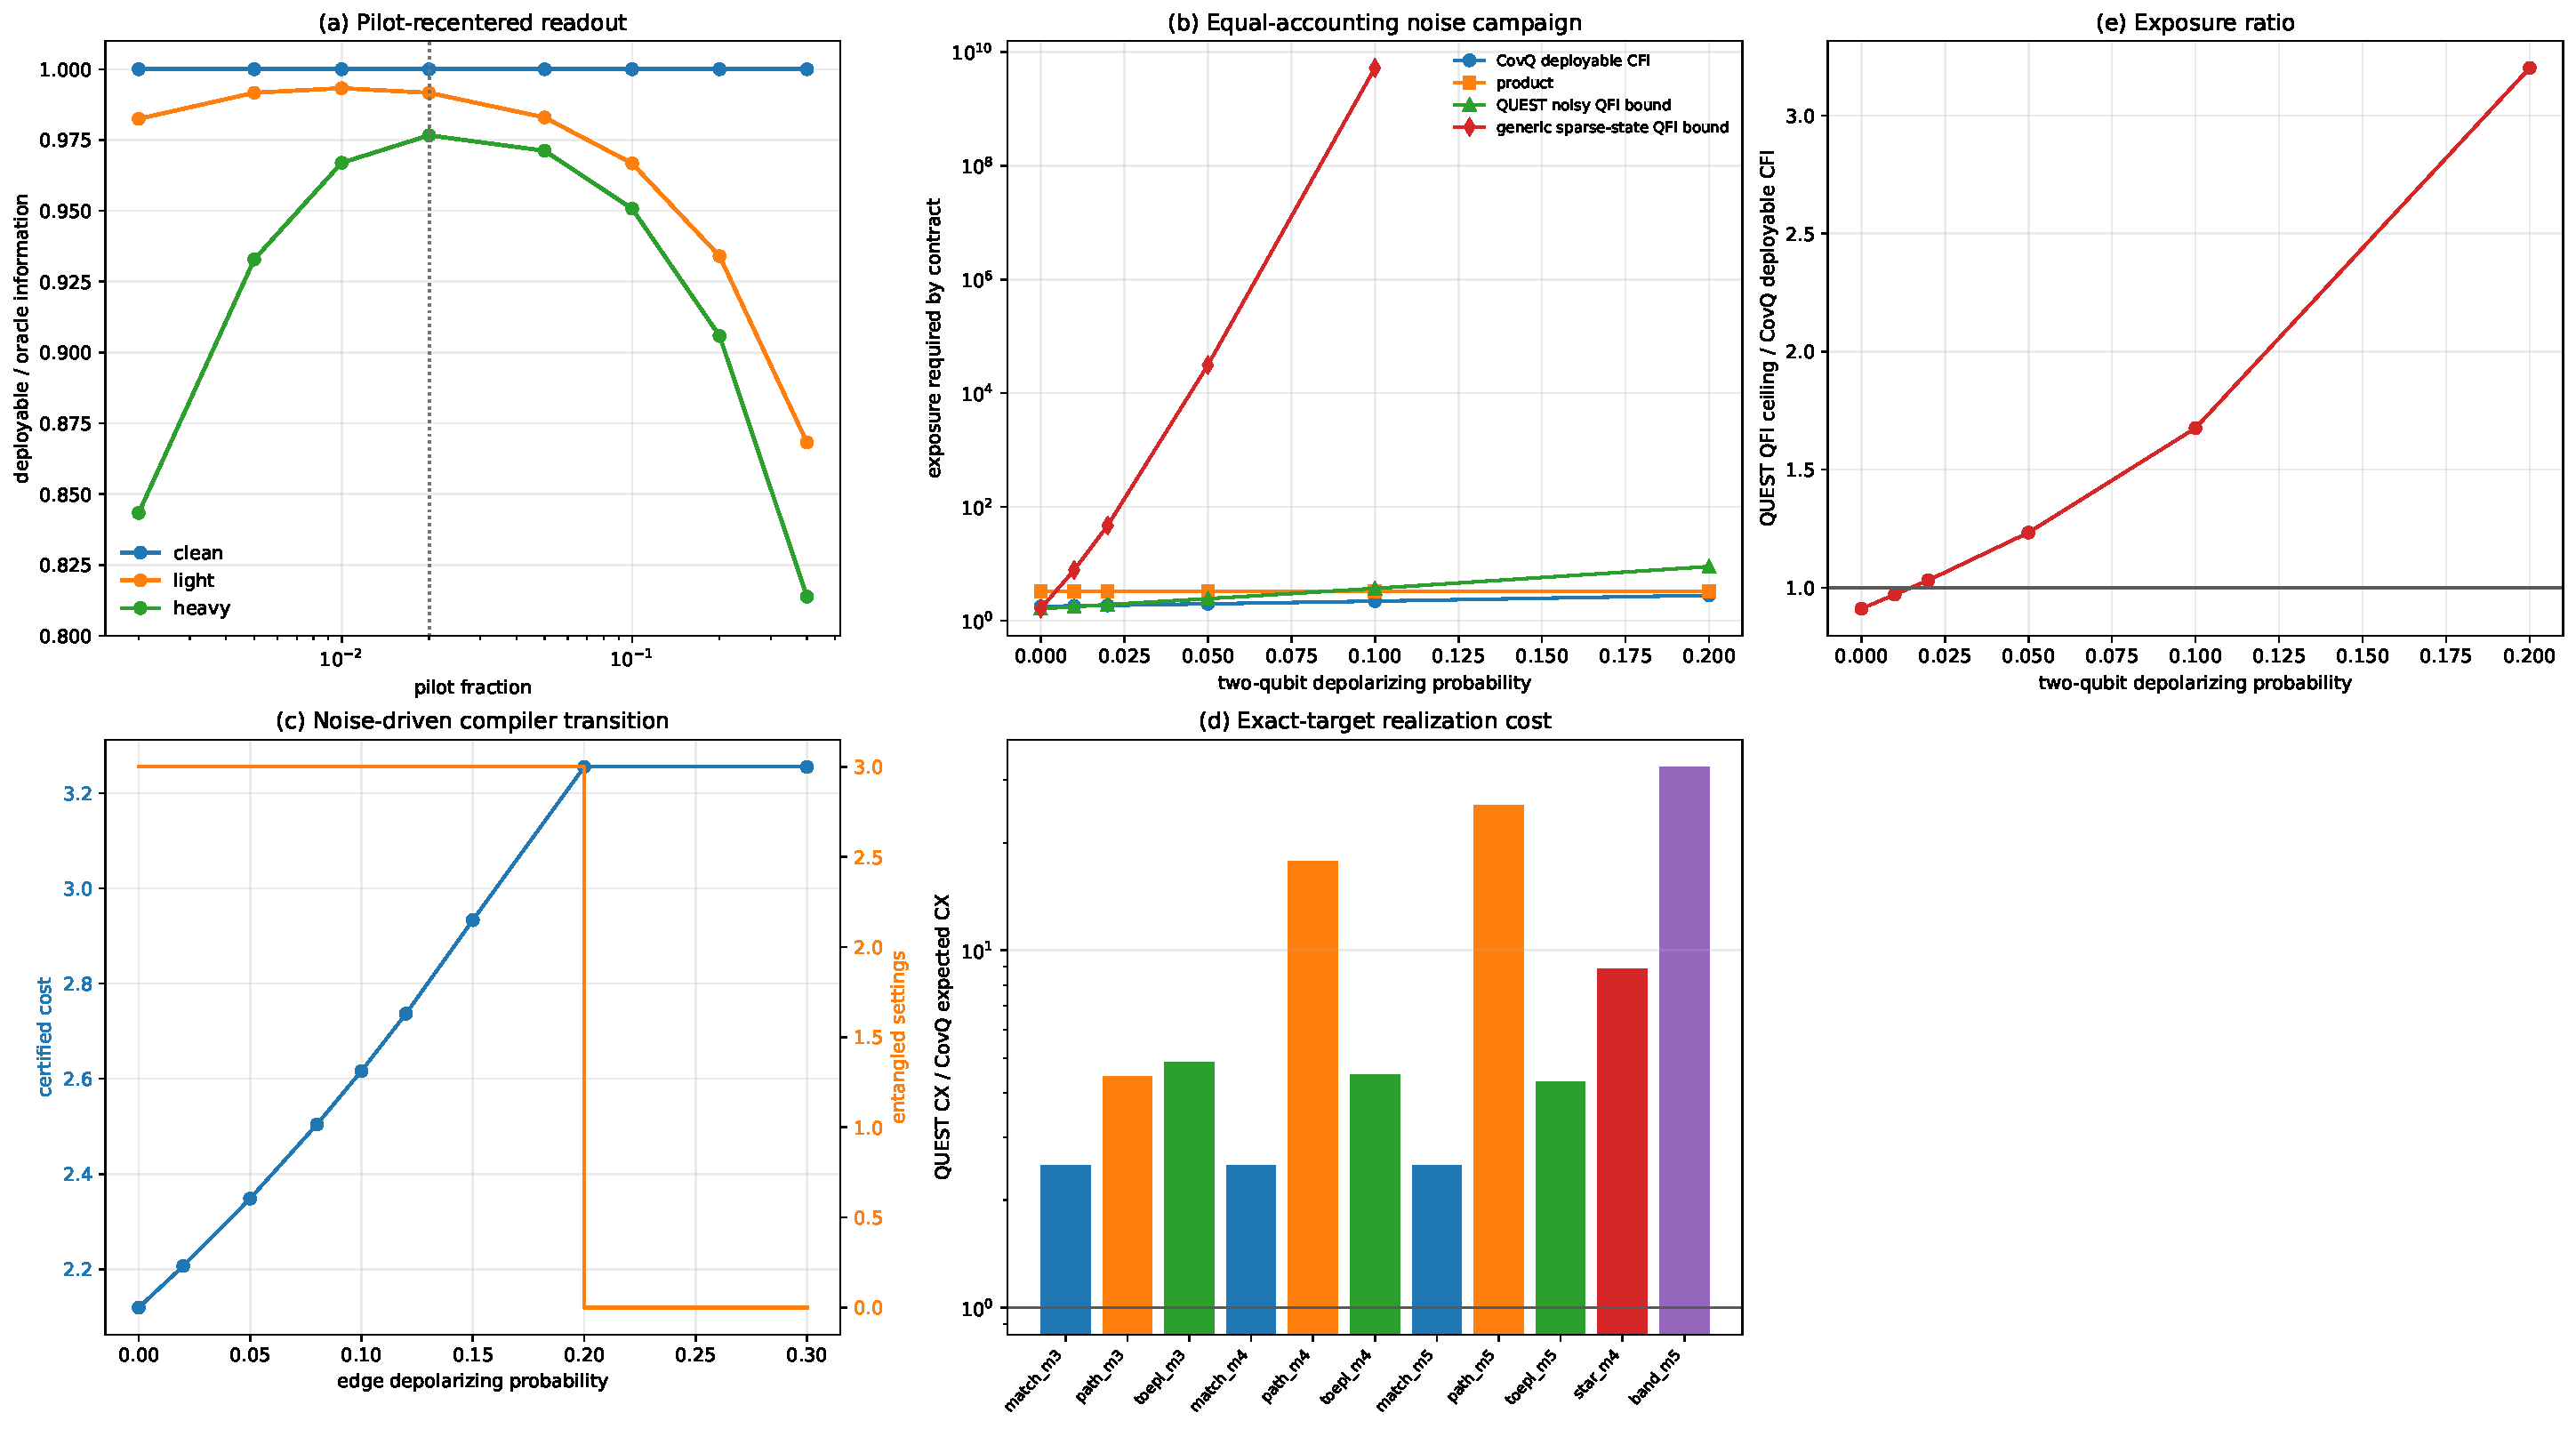
\includegraphics[width=\textwidth]{operational_results.pdf}
  \caption{Operational results. (a) Pilot-recentered information relative to the true-analyzer oracle; the vertical line marks the frozen cross-regime $f=0.02$ policy. (b) Required exposure in the equal-accounting noisy contract campaign; QUEST and sparse one-state curves are optimistic QFI bounds. (c) The noise-aware compiler uses three entangled settings through the tested $0.15$ point and switches to one pairless setting at $0.20$. (d) QUEST/CovQ expected-CX ratio on exact targets; modest matching/Toeplitz cases and large path/star/banded separations coexist.}
  \label{fig:operational-results}
\end{figure}

\subsection{Fixed-setting greedy selection fails}
\label{sec:results-fixed-settings}
The fixed-setting extension is nonconvex, and the tested greedy forward heuristic fails exactly where multi-setting schedules matter. Table~\ref{tab:n9} and \cref{fig:n9} compare it with exhaustive support enumeration on the registered small instance.

\begin{table}[H]
\centering
\caption{Fixed-setting penalty experiment.}
\label{tab:n9}
\begin{tabular}{rrrrrr}
\toprule
$\lambda_q$ & greedy cost & $q_g$ & exact cost & $q_\star$ & excess\\
\midrule
0.0 & 2.27865 & 1 & 2.12480 & 2 & 7.24\%\\
0.1 & 2.37865 & 1 & 2.32480 & 2 & 2.32\%\\
0.2 & 2.47865 & 1 & 2.47865 & 1 & 0\\
0.3 & 2.57865 & 1 & 2.57865 & 1 & 0\\
1.0 & 3.27865 & 1 & 3.27865 & 1 & 0\\
\bottomrule
\end{tabular}
\end{table}

\begin{figure}[H]
  \centering
  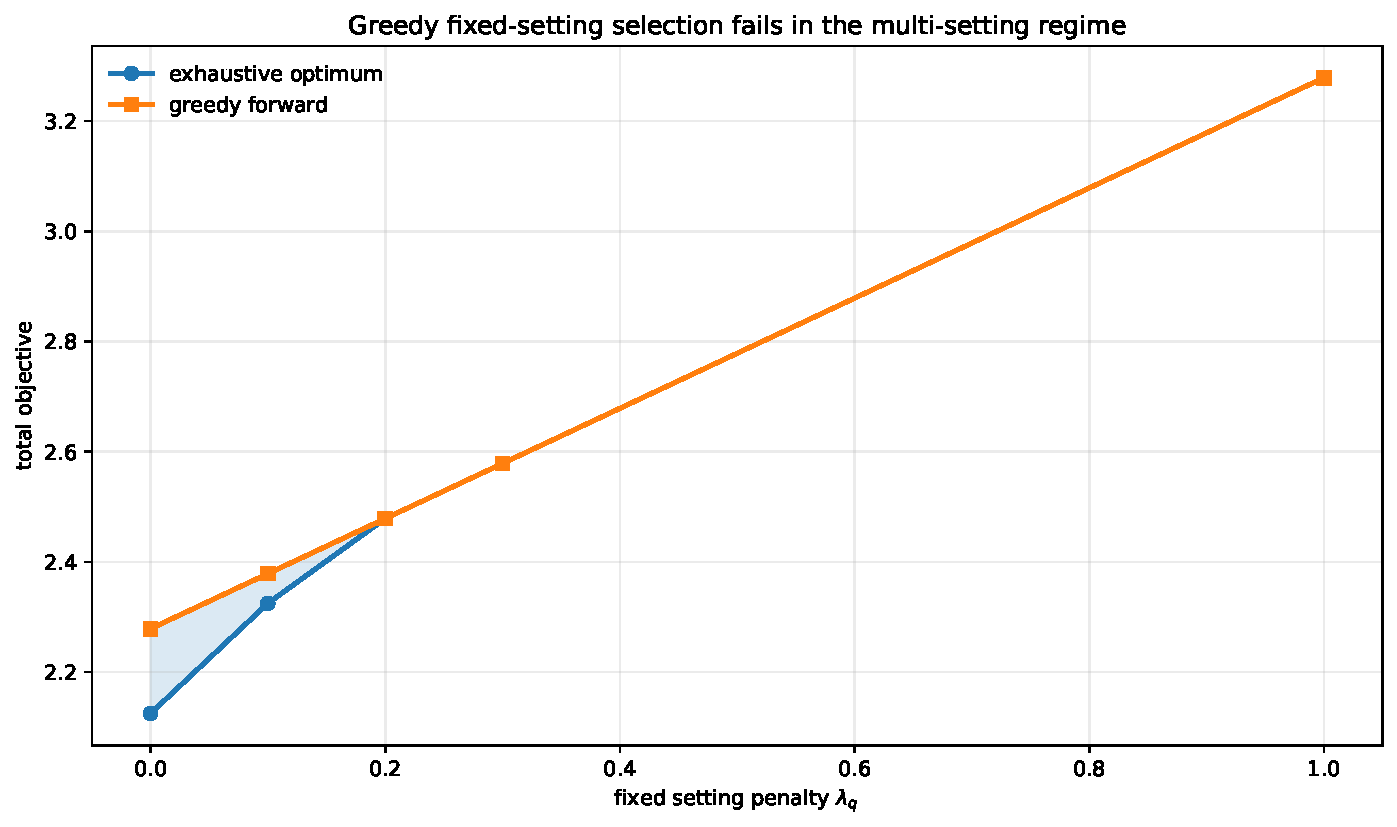
\includegraphics[width=0.86\textwidth]{fixed_setting_failure.pdf}
  \caption{Greedy forward selection becomes exact only after the cardinality penalty has made a one-setting solution optimal. It is therefore retained as a labeled heuristic, not an exact fixed-charge compiler.}
  \label{fig:n9}
\end{figure}

\subsection{Setting-cost amortization}
CovQ's extra configurations can be priced rather than left as an unquantified caveat. Under batched switching, the exact-target crossover is given by \cref{eq:setting-crossover}. With a deliberately pessimistic setup charge of $10^4$ two-qubit-gate equivalents, the worst registered crossover was approximately $1.30\times10^4$ shots; structured path, star, and banded targets crossed in a few hundred shots or fewer. This analysis does not turn the convex compiler into a fixed-charge optimum. It states the repetition count above which per-shot circuit savings amortize configuration overhead.

\subsection{Artifact status}
All scientific arms required for the paper's current scope are now present: exact pair geometry, certificates, operational readout, estimator, adaptive recentering, block-local noisy pricing, QUEST comparison, settings amortization, and the N9 negative result. The remaining issue is archival provenance. The integrated commit reports 156 passing tests, but the result files still identify earlier source commits and a dirty tree. No number in this section should be considered journal-archival until the clean release rerun described in Appendix~\ref{app:release-checklist} reproduces it without changing the frozen configuration.


\section{Illustrative application interface: Lorentzian light-ray tomography}
\label{sec:application}

The paper remains a quantum-compilation paper if this section is deleted. The Lorentzian application is included because it makes the downstream-map interface concrete and was the source of the original companion-study question.

\subsection{The application is exactly a Fisher-information contract}
For a finite metric parameter vector $\bm\theta$, Paper~1 gives link parameters $x=J\bm\theta$, a link-level probe-information matrix $W_\rho$, and the pullback
\begin{equation}
  F_{\bm\theta}=J^{\mathsf T}W_\rho J.
  \label{eq:light-ray-pullback}
\end{equation}
That work executes independent probes and leaves correlated link-QFIM design to a companion study~\cite{DixitChauhan2026}. CovQ supplies the program layer by setting
\begin{equation}
  F_{\PiProg}=W_\rho,
  \qquad A=J,
\end{equation}
so that the user-facing contract is
\begin{equation}
\boxed{
  J^{\mathsf T}F_{\PiProg}J\succeq G_{\theta,{\rm req}}.}
  \label{eq:spacetime-floor}
\end{equation}
Many link-level QFIMs can satisfy the same metric-level requirement; choosing the cheapest one is precisely the freedom the information-floor compiler is designed to exploit.

\subsection{The geometric kernel remains absolute}
For every positive semidefinite probe-information matrix,
\begin{equation}
  \ker J\subseteq\ker(J^{\mathsf T}F_{\PiProg}J).
  \label{eq:application-nonlifting}
\end{equation}
CovQ can redistribute information only on $\im J$. A different physical observable changes $J$; entanglement or schedule design changes $F_{\PiProg}$. The application must therefore compile on an identified quotient or declared visible support and cannot use a quantum program to manufacture information absent from the light-ray channel.

\subsection{Status of this interface}
No new light-ray numerical campaign is used to support the CovQ theorems or the comparative claims in \cref{sec:results}. A future application package need only ingest a committed Jacobian, parameter metric, visible support, hardware graph, and metric-level floor, then run the same certified compiler. Keeping that work separate prevents spacetime-specific modeling choices from becoming hidden assumptions of the quantum compiler.


\section{Limitations and open problems}
\label{sec:limitations}

\subsection{Exact scope of the reachable-body theorem}
The exact matching characterization assumes independent commuting Pauli generators, retained classical branch labels, physical-$Z$ normalization for the direct hardware theorem, and block-product branches of width at most two. Dependent generators restrict the joint sign patterns to a binary code. Noncommuting generators introduce complex tangent geometry and measurement incompatibility. Neither extension follows by mechanically replacing the edge set.

\subsection{Program width is instruction-set relative}
Labeled branch width is exact for the declared pair-block instruction set. It is not a universal minimum over analog global gates, measurement-based preparation, fault-tolerant encodings, or coherent flag-data purifications. Clifford normalization preserves QFIM semantics but can make the physical state globally entangled, so logical width, physical entanglement, frame cost, and routing cost remain separate ledger entries.

\subsection{Block-local noise is a real restriction}
The noisy matching theorem excludes crosstalk, correlated branch noise, route collisions, coherent errors spanning blocks, and cardinality-dependent depth. Under those effects, edge additivity can fail and pricing need not remain matching. The paper therefore claims an exact block-local noisy compiler, not a universal noise-aware reduction.

\subsection{One-state baselines are not fully operational}
QUEST is given its noisy QFI as an optimistic upper bound because no attaining noisy multiparameter readout was compiled. CovQ is evaluated with an emitted readout. A CovQ win under that asymmetry is strong; a QUEST upper-bound win would not establish operational superiority. The generic sparse Carath\'eodory circuit uses 232 CX gates and is explicitly a synthesis upper bound. The paper does not claim to defeat an optimized support-aware sparse-state compiler.

\subsection{Fixed setting charges remain nonconvex}
The exact compiler minimizes additive execution cost. Fixed per-configuration charges create a mixed-integer conic problem. Exhaustive support enumeration is exact only at small scale, and the tested greedy heuristic fails by $7.24\%$ in the multi-setting regime. The manuscript therefore reports an amortization boundary, not a globally minimum fixed-charge schedule.

\subsection{Adaptive readout and periodic identifiability}
The analyzer-phase pilot removes the true-state oracle in the registered phase-covariant model and supplies an initialization chart for the periodic likelihood. The release policy freezes $f=0.02$, but a detector-facing implementation should calibrate the visibility class, analyzer offset, and drift model independently. At zero contrast the phase is undefined and no readout can recover information. Global identifiability remains modulo the physical phase periodicity and the QFIM kernel.

\subsection{Finite schedules and finite samples}
The conic compiler returns real exposures. Finite campaigns round or sample branch counts. Tight contracts can therefore require a robust surplus margin and concentration analysis. The current estimator experiments demonstrate local efficiency on registered small instances; they do not constitute a uniform finite-sample theorem for every contract.

\subsection{Simulation and repository scale}
The numerical work is a certified prototype, not a hardware demonstration. Exact-target comparisons use $m\le5$, and the principal noisy contract uses four generators. The polynomial matching oracle and theorem apply beyond this surface, but wall-clock scaling, hardware calibration, and route-aware execution are not claimed. A journal presentation should be read as theory plus reproducible compiler validation.

\subsection{Novelty remains falsifiable}
CovQ does not claim expectation targeting, optimal design, correlation polytopes, matching algorithms, Bell preparation, or entanglement witnessing as new. The scoped claim is their end-to-end composition into a downstream information-floor compiler with an exact pair-width reachable body, emitted circuits and readout, and certificates. Discovery of prior work solving that same composite input-output problem would require another narrowing.

\section{Conclusion}

CovQ turns a downstream Fisher-information requirement into an executable quantum experiment. Its primary output is not merely a state or an ideal QFIM: it is an exposure-weighted retained-label schedule, native preparation circuits, a pilot policy, an ancilla-free local readout, a parity likelihood, an estimator, and a primal--dual certificate satisfying the requested information floor.

The exact pair-width reachable body is the compiler engine. For physical commuting $Z_i/2$ generators on a hardware graph, a unit-diagonal QFIM is achievable by labeled pair-width programs exactly when its nonedge correlations vanish and its edge magnitudes lie in the matching polytope. That quantum identification makes signs independently realizable, turns matching decompositions into depth-one Bell schedules, and gives expected pair activation a literal circuit meaning. The width-three boundary explains why the tractable regime is special rather than the first step of an automatic hierarchy.

The operational layer is now closed for the principal backend. Local equatorial measurements attain every emitted signed-cat block, parity is sufficient, a branch-conditioned MLE is empirically efficient, and a two-quadrature pilot selects the correct periodic likelihood chart. Under generator-basis pinching, covariance can remain unchanged while all QFI and operational information disappear, so the noisy compiler correctly uses declared-readout CFI rather than covariance.

Block-local noise preserves the matching combinatorics while changing edge values and the optimal program. In the registered contract, the compiler moved from three entangled settings to one product setting as edge noise increased. Against a faithful QUEST reimplementation, the results reveal a phase diagram rather than universal dominance: the one-state realization is more shot efficient in the noiseless row, while CovQ's depth-one schedules require less exposure at every tested edge-depolarization point from $1\%$ onward under an accounting deliberately favorable to QUEST. Extra settings are governed by an explicit amortization boundary. The fixed-setting greedy method fails and remains a negative result.

The scientific program is therefore ready to stop expanding. The remaining work is release engineering, independent proof reading, manuscript compression, citation checking, and journal formatting. New Clifford, coherent-flag, crosstalk, routing, or hardware studies would be valuable follow-on work, but they are not required to support the present theorem-and-compiler paper.

\appendix

\section{Notation and implementation conventions}

\begin{table}[H]
\centering
\caption{Core notation.}
\begin{tabularx}{\textwidth}{p{0.20\textwidth}X}
\toprule
$P_i$ & Commuting Pauli generator with $P_i^2=I$.\\
$F$ & QFIM in the normalization $U_{\bm\theta}=\exp[-\tfrac i2\sum_i\theta_iP_i]$.\\
$H=(V,E)$ & Direct hardware coupling graph for the pair backend.\\
$M$ & Matching of $H$.\\
$\sigma_e$ & Sign selecting $\ket{\Phi^+}$ or $\ket{\Psi^+}$ on edge $e$.\\
$B_{M,\sigma}$ & Unit-diagonal signed-matching branch QFIM.\\
$\Q^{\lab}_{H,2}$ & Feasible QFIMs of retained-label direct pair-width programs.\\
$\mathcal C_m$ & Full symmetric-Bernoulli correlation polytope.\\
$A$ & Downstream parameter map in the contract $A^{\mathsf T}FA\succeq G_{\rm req}$.\\
$G_{\rm req}$ & Required downstream Fisher-information floor.\\
$t_e$ & Auxiliary native-edge magnitude/load variable; an optimum has $t_e=|F_e|$.\\
$Y,\beta$ & Dual PSD witness and scalar normalization for minimum-cost certification.\\
\bottomrule
\end{tabularx}
\end{table}

Computational basis labels use $s_i=+1$ for $\ket0$ and $s_i=-1$ for $\ket1$. Matrix inner products use $\langle A,B\rangle=\tr(A^{\mathsf T}B)$. Every symmetric off-diagonal edge therefore contributes twice to the matrix inner product, explaining the factor two in matching weights.

\section{Proof details for the coherent-flag formula}

For completeness, write
\begin{equation}
  M_r=F_r+\bm\mu_r\bm\mu_r^{\mathsf T}.
\end{equation}
The global flagged second moment is $\overline M=\sum_rp_rM_r$, while the global mean is $\overline{\bm\mu}$. Therefore
\begin{align}
  F_{\coh}
  &=\overline M-\overline{\bm\mu}\,\overline{\bm\mu}^{\mathsf T}\\
  &=\sum_rp_rF_r+
  \sum_rp_r\bm\mu_r\bm\mu_r^{\mathsf T}
  -\overline{\bm\mu}\,\overline{\bm\mu}^{\mathsf T}.
\end{align}
This derivation also shows why measuring the flag is not a harmless implementation detail. Dephasing removes cross-branch amplitude coherence before the QFI optimization and returns the classical--quantum direct sum.

\section{Proof details for matching necessity}

A vector $a$ supported on a matching $M$ with $0\le a_e\le1$ lies in $\MATCH(H)$. One explicit decomposition is obtained by independently including edge $e\in M$ with probability $a_e$. Every outcome is a submatching of $M$, and its expected incidence vector is $a$. This avoids assuming that a two-qubit branch correlation is already extremal.

Down-monotonicity follows directly from Edmonds' description: all nontrivial inequalities have nonnegative coefficients and upper bounds. It also follows probabilistically by thinning a random matching edgewise.

\section{A small exact example}

Let $H=K_3$ and
\begin{equation}
  F=\begin{pmatrix}
  1&0.4&-0.3\\
  0.4&1&0.2\\
  -0.3&0.2&1
  \end{pmatrix}.
\end{equation}
The magnitude vector is $(0.4,0.3,0.2)$ and satisfies the triangle odd-set load $0.9\le1$. One matching decomposition is
\begin{align}
  0.4\,\chi^{\{12\}}
  +0.3\,\chi^{\{13\}}
  +0.2\,\chi^{\{23\}}
  +0.1\,\chi^{\varnothing}.
\end{align}
The compiler emits four branches: $\ket{\Phi^+}_{12}\ket{+}_3$, $\ket{\Psi^+}_{13}\ket{+}_2$, $\ket{\Phi^+}_{23}\ket{+}_1$, and $\ket{+}^{\otimes3}$ with the displayed probabilities. The expected active-pair cost is $0.9$, exactly $|0.4|+|-0.3|+|0.2|$.

By contrast, replacing the magnitudes with $(0.5,0.5,0.5)$ violates the odd-set bound by $0.5$. Proposition~\ref{prop:distance-certificate} yields the Frobenius lower bound
\begin{equation}
  \dist_F(F,\Q^{\lab}_{K_3,2})
  \ge\sqrt2\frac{0.5}{\sqrt3}\approx0.408.
\end{equation}


\section{Repository result schema and provenance}
\label{app:result-schema}

Every canonical result record contains at least:
\begin{lstlisting}[style=covqcode,language={}]
{
  "schema_version": "covq.measurement.record/0.1",
  "source_commit": "<final release sha>",
  "dirty": false,
  "config_sha256": "<sha256>",
  "environment": {...},
  "gate": "<gate id>",
  "status": "DONE|FAILS|ABSENT",
  "inputs": {...},
  "circuits": {"hashes": [...], "resources": [...]},
  "ideal_qfim": [...],
  "mixed_state_qfim": [...],
  "declared_readout_cfi": [...],
  "primal_cost": "<number or null>",
  "dual_bound": "<number or null>",
  "optimality_gap": "<number or null>",
  "record_hash": "<sha256>"
}
\end{lstlisting}
The current development records preserve the correct numerical payloads but identify earlier source commits and a dirty tree. The journal release must regenerate, not hand-edit, these fields.

The principal records are:
\begin{itemize}
  \item \texttt{results/measurements/ideal\_block\_readout.json};
  \item \texttt{results/measurements/schedule\_attainability.json};
  \item \texttt{results/measurements/estimator\_efficiency.json};
  \item \texttt{results/noise/adaptive\_readout\_performance.json};
  \item \texttt{results/noise/noise\_aware\_floor\_compiler.json};
  \item \texttt{results/noise/noisy\_pricing\_oracle.json};
  \item \texttt{results/noise/quest\_operational\_comparison.json};
  \item \texttt{results/noise/fixed\_setting\_cost\_solver.json};
  \item \texttt{results/noise/setting\_cost\_phase\_diagram.json};
  \item \texttt{results/baselines\_k3\_quest.json}.
\end{itemize}
Every paper table and figure is generated from these artifacts. Manual transcription is permitted only for proof statements, never for numerical results.

\section{Journal release checklist}
\label{app:release-checklist}

The research scope is frozen. Before submission, the release agent must complete the following finite checklist without adding a new scientific arm.

\begin{enumerate}[label=\textbf{R\arabic*.}]
  \item Freeze one release commit and tag; vendor the exact manuscript, bibliography, configuration, environment lock, and figure-generation scripts.
  \item Add an independent mixed-state QFIM regression by solving the SLD equations and comparing with \cref{eq:mixed-qfim-spectral} on random complex mixed states.
  \item Freeze the deployable pilot policy at $f=0.02$ and regenerate the N7 and N10 records under that policy; retain the per-regime best-$f$ sweep as an oracle diagnostic.
  \item Run the full 156-test suite plus the new SLD regression from a clean checkout on the primary platform. Run the compact correctness suite on a second operating system or Python environment.
  \item Regenerate every canonical record with the final source SHA and \texttt{dirty: false}; fail closed if any numerical payload changes outside the registered tolerance.
  \item Rebuild all manuscript tables and figures only from the regenerated records and compare them against this draft.
  \item Preserve N9 as \texttt{FAILS}; do not claim exact optimization of fixed configuration charges.
  \item Preserve the sparse-state caveat; do not rename the 232-CX generic-synthesis upper bound as an optimized sparse baseline.
  \item Describe QUEST's noisy column as an optimistic QFI upper bound with no compiled attaining readout.
  \item Obtain an independent line-by-line proof audit of the matching theorem, coherent-flag identity, shot-scaled dual, noisy matching theorem, and width-three reduction.
  \item Run citation and title checks through the submission date, especially for QUEST, the 2026 correlation-polyhedron hardness result, and QFIM entanglement literature.
  \item Compile the PDF twice from a clean source bundle, preflight it, render every page, and verify equations, tables, figures, links, and fonts.
  \item Mint an archival repository release and DOI; record SHA-256 hashes for source, environment, canonical results, and PDF.
  \item Remove ``journal-preparation'' and replace it with the final version/date only after R1--R13 pass.
\end{enumerate}

\begin{claimbox}[title={Submission decision}]
Completion of R1--R14 is sufficient to move this manuscript into journal submission and polishing. None of the open extensions---Clifford-frame readout cost, coherent-flag joint readout, routing, crosstalk, or real-hardware execution---is required for the scoped theory-and-compiler claim. If a release rerun changes a headline result beyond tolerance, submission pauses and the discrepancy is investigated; otherwise the research campaign stops.
\end{claimbox}

\printbibliography

\end{document}
